% Carattere dimensione 12
\documentclass[12pt]{report}

% Per la stampa fronte-retro sostituire con:
%\documentclass[12pt, twoside]{report}

% Margini (4cm a sx, 2.5cm a dx, 2.5cm in alto, 2.5cm in basso)
\usepackage[top=2.5cm, bottom=2.5cm, left=4cm, right=2.5cm, centering, head=21.75 pt]{geometry}

% Per la stampa fronte-retro sostituire con: 
%\usepackage[top=2.5cm, bottom=2.5cm, inner=4cm, outer=4cm, right=2.5cm, centering]{geometry}

% Interlinea
\linespread{1.5}

% Librerie utili

\usepackage{amsmath} % AMS Math Package
\usepackage{amsthm} % Theorem Formatting
\usepackage{subfig}
\usepackage{booktabs}


\usepackage{amssymb}
\usepackage{enumitem}


\usepackage{physics}   %for bra ket notation
 
\usepackage[italian]{babel} % applicazione regole di scrittura per la lingua italiana 
\usepackage[utf8]{inputenc} % codifica UTF-8
\usepackage{scrlayer-scrpage} % stili pagina per il frontespizio
\ifoot[]{}
\cfoot[]{}
\ofoot[\pagemark]{\pagemark}
\pagestyle{scrplain}
%\usepackage{mathptmx} % font Times New Roman (simile)
\usepackage{graphicx} % inserimento di immagini
\usepackage{csquotes} % per le citazioni "in blocco"
\usepackage[backend=biber, sorting=none, ]{biblatex} % bibliografia con pacchetto biblatex (https://ctan.org/pkg/biblatex?lang=en)
\appto{\bibsetup}{\raggedright}
\addbibresource{bibliography.bib}

\usepackage{titlesec} % per la formattazione dei titoli delle sezioni, capitoli etc.
\usepackage{float} % per il posizionamento delle immagini

\usepackage{nicefrac}

\usepackage{listings} % per il codice di programmazione
% Fonte https://en.wikibooks.org/wiki/LaTeX/Source_Code_Listings. Per la lista di sintassi riconosciute.
\renewcommand{\lstlistingname}{Code}% Listing -> Codice
\usepackage{xcolor}  % stile del codice
\definecolor{mygreen}{rgb}{0,0.6,0}
\definecolor{mygray}{rgb}{0.5,0.5,0.5}
\definecolor{mymauve}{rgb}{0.58,0,0.82}
\definecolor{darkgray}{rgb}{.4,.4,.4}
\definecolor{navy}{HTML}{000080}
\definecolor{purple}{rgb}{0.65, 0.12, 0.82}
\definecolor{codepurple}{rgb}{0.58,0,0.82}
\definecolor{backcolour}{rgb}{0.95,0.95,0.92}

\definecolor{codegreen}{rgb}{0,0.6,0}
\definecolor{codegray}{rgb}{0.5,0.5,0.5}
\definecolor{codepurple}{rgb}{0.58,0,0.82}
\definecolor{backcolour}{rgb}{0.95,0.95,0.92}

\lstdefinestyle{mystyle}{
    backgroundcolor=\color{backcolour},   
    commentstyle=\color{codegreen},
    keywordstyle=\color{magenta},
    numberstyle=\tiny\color{codegray},
    stringstyle=\color{codepurple},
    basicstyle=\ttfamily\footnotesize,
    breakatwhitespace=false,         
    breaklines=true,                 
    captionpos=b,                    
    keepspaces=true,                 
    numbers=left,                    
    numbersep=5pt,                  
    showspaces=false,                
    showstringspaces=false,
    showtabs=false,                  
    tabsize=2
}

\lstset{style=mystyle}

\definecolor{dark-gray}{gray}{0.2}
\usepackage[font=footnotesize, justification = centering, labelfont = {color = dark-gray}]{caption} %, figurename = Fig.
\usepackage{hyperref}   %link pdf
\usepackage{setspace}

% Formato delle intestazioni
\titleformat{\chapter}[block]
  {\normalfont\LARGE\bfseries}{\thechapter.}{0.5em}{\LARGE}
\titlespacing*{\chapter}{0pt}{-20pt}{25pt}

\begin{document}

% Frontespizio
\begin{titlepage}
\begin{center}
    {\LARGE{Università degli Studi di Milano-Bicocca \\}}
    {\small{Dipartimento di Fisica}}\\
    {\small{Corso di Laurea Triennale}}
\end{center}
    
\begin{figure}[H]
    \centering
    
\includegraphics[width=0.4\textwidth]{logo.png}
\end{figure}

\vspace{0.5cm}


\begin{center}
    {\huge {Soluzione numerica dell'equazione di Schr\"odinger}}
\end{center}

\vspace{2cm}

\begin{minipage}[t]{0.47\textwidth}
	{\large{\bf Relatore:\\ Carlo Oleari}}
	%\vspace{0.5cm}
	%{\large{\bf \\Correlatore:\\ Nome Cognome}}
\end{minipage}\hfill\begin{minipage}[t]{0.47\textwidth}\raggedleft
	{\large{\bf Candidato: \\Luca Falzoni\\ }}
\end{minipage}

\vspace{25mm}

\centering{\large{\bf ANNO ACCADEMICO 2021/2022 }}
\end{titlepage}
% Fine frontespizio


\begin{spacing}{1.4}
    \tableofcontents
\end{spacing} 
\thispagestyle{empty}

%\listoffigures

\thispagestyle{empty}
\clearpage
\setcounter{page}{1}
\addtocontents{toc}{\protect\thispagestyle{empty}}
\addcontentsline{toc}{chapter}{Introduzione} % Capitolo non numerato

\chapter*{Introduzione}
\label{ch:introduzione}

La soluzione esatta dell'equazione di Schr\"odinger, 
\begin{equation}
    \centering
    i \hbar \frac{\partial}{\partial t} \psi (\vec{x}, t) = \hat{H} (\vec{x}, t) \psi (\vec{x}, t) \; \text{,}
    \label{eq:Sc}
\end{equation}
può essere espressa in termini di funzioni semplici solo per un numero ristretto di problemi. Per fare previsioni e ottenere risultati concreti, è quindi di fondamentale importanza utilizzare metodi di soluzione numerici.

Si propone un metodo per la soluzione numerica dell'eq.(\ref{eq:Sc}) che consiste nell'applicazione ripetuta dell'espressione infinitesima dell'operatore di evoluzione temporale, approssimato tramite l'espansione di  Lie-Trotter.

È stato sviluppato un software che consiste di tre componenti principali: 
\begin{itemize} [nolistsep, leftmargin=1.5cm]
    \item un ambiente grafico per poter gestire i parametri della simulazione,
    \item l'algoritmo simulativo,
    \item una serie di strumenti grafici per mostrare i risultati tramite animazioni.
\end{itemize}

Il metodo è stato innanzitutto validato tramite il confronto delle simulazioni con alcune soluzione esatte, tra cui il problema di particella libera, la dinamica degli stati coerenti dell'oscillatore armonico e, nel potenziale di P\"oschl-Teller, l'evoluzione di un pacchetto gaussiano di autostati. In seguito, si è utilizzato il software per risolvere alcuni dei problemi monodimensionali generalmente proposti nei corsi di meccanica quantistica e altri di particolare interesse.

\chapter{L'equazione di Schr\"odinger}
\label{ch:eqS}

La più generica forma dell'equazione di Schr\"odinger risulta essere quella nell'eq.(\ref{eq:Sc}), dove $\hat{H}$ rappresenta l'operatore Hamiltoniano  \footnote{Si ricorda che le grandezze riportate sotto il simbolo $\, \hat{ } \,$ rapprenatano degli operatori lineari in uno spazio di Hilbert.}
\begin{equation}
    \centering
    \hat{H} (\vec{x}, t) = \frac{1}{2m} \left[\hat{p} - q \hat{A}(\vec{x}, t) \right]^2 + \hat{V}(\vec{x}, t) - g \frac{q}{2m} \hat{S} \cdot \hat{B}(\vec{x},t) \; \text{.}
    \label{eq:H}
\end{equation}
Di seguito, nei casi presi in esame, si utilizza una forma semplificata dell'eq.(\ref{eq:Sc}) e dell'operatore nell'eq.(\ref{eq:H}), poiché verranno utilizzati nella loro forma monodimensionale e senza considerare interazioni di natura elettromagnetica. Questa semplificazione non modifica il formalismo matematico utilizzato, ma permette di rendere più esplicative e chiare le espressioni che seguiranno. È dunque possibile riadattare tali espressioni e generalizzarle utilizzando lo stesso procedimento. L'equazione risolta nelle simulazioni risulta essere
\begin{equation}
    \centering
    i \hbar \frac{\partial}{\partial t} \psi (x, t) =  \hat{H} (\vec{x}, t) \psi (\vec{x}, t)   \qquad \text{con} \quad \hat{H} (\vec{x}, t) = \frac{\hat{p}^2}{2m}  + \hat{V}(\vec{x}, t) = \hat{T} + \hat{V} \; \text{,}
    \label{eq:Sc_1D}
\end{equation}
dove si ricorda che, nella rappresentazione delle coordinate, 
\begin{equation}
    \centering
    \hat{p}_{x} = - i \hbar \frac{\partial } {\partial x} \; \text{.}
    \label{eq:p}
\end{equation}
La soluzione formale dell'equazione di Schr\"odinger fa uso dell'operatore unitario di evoluzione temporale 
\begin{equation}
    \centering
    \psi (x,t) = \hat{U}(t, t_{0}) \, \psi (x, t_0) \quad \text{con} \quad \hat{U}(t, t_{0}) = \hat{T}  \exp \left[\frac{-i}{\hbar} \int _{t_{0}} ^{t} dt' \; \hat{H}(x,t') \right] \; \text{,}
    \label{eq:U}
\end{equation}
dove $\hat{T}$ è l'operatore di prodotto T-ordinato. Per semplicità di notazione non si è riportata la dipendenza di $\hat{U}$ da $\hat{x}$. 
% Devo paarlare del motivo per cui viene semplicata
Tale soluzione, non essendo esplicitamente analitica, non può essere risolta in maniera esatta se non in casi molto particolari.
Se però si considera l'espressione infinititesima dell'operatore $\hat{U}$, risulta
\begin{equation}
    \centering
    \hat{U}(t + \delta t, t) = \exp \left[\frac{-i}{\hbar} {H}(x,t) \delta t \right]  \; \text{,}
    \label{eq:U_inf}
\end{equation}
che può essere applicato senza difficoltà alla funzione d'onda $\psi(x,t)$ un numero di volte necessarie a ottenere lo stesso risultato dell'eq.(\ref{eq:U}).
L'unica difficoltà risiede nell'espansione dell'operatore, poiché in forma esplicita  
\begin{equation}
    \centering
    \hat{U}(t + \delta t, t) =  \exp \left[\frac{-i}{\hbar} \delta t (\hat{V} + \hat{T}) \right] \; \text{,}
    \label{eq:U_esplicit} 
\end{equation}
dove $\hat{V}$ e $\hat{T}$ sono due operatori che non commutano. Questo rende l'espansione dell'operatore $\hat{U}$ non banale.

\clearpage

\chapter{Metodo}
\label{ch:teoria}

Nel seguente capitolo vengono esposti gli aspetti teorici utili nella comprensione del modello, degli strumenti utilizzati e delle condizioni imposte dalla simulazione sulla natura del sistema.

\section{Espansione di Lie-Trotter}
\label{sec:LT}

Per espandere l'operatore, si è scelto di utilizzare un risultato noto con il nome di ``Formula di Lie-Trotter"
\begin{equation}
    \centering
     \exp \left(\hat{A} + \hat{B}\right) = \lim_{n\to\infty } \left[  \exp \left(\frac{\hat{A}}{n}\right)  \exp \left(\frac{\hat{B}}{n}\right) \right] ^{n} \; \text{,}
    \label{eq:LT_formula}
\end{equation}
dove $\hat{A}$ e $\hat{B}$ rappresentano due generici operatori lineari non commutanti.
Dall'eq.(\ref{eq:LT_formula}) si può dimostrare che vale la seguente espansione 
\begin{equation}
    \centering
    \exp \left[\tau (\hat{A} + \hat{B})\right]
    = \prod _{j=1} ^{n}  \exp \left( \tau \hat{A} c_{j}\right)   \exp \left(\tau \hat{B} d_{j}\right) + \mathcal{O}(\tau^{n+1}) \; \text{,}
    \label{eq:LT_expantion}
\end{equation}
con $c_{i}$ e $d_{i}$ coefficienti reali.

All'interno del codice sono stati implementai tre diversi livelli di profondità, troncando la produttoria al primo ordine
\begin{equation}
    \centering
    \exp \left[\tau (\hat{A} + \hat{B})\right]
    =  \exp \left( \tau \hat{A} \right)   \exp \left(\tau \hat{B} \right) + \mathcal{O}(\tau^{2}) \; \text{,}
    \label{eq:LT_1}
\end{equation}
al secondo ordine 
\begin{equation}
    \centering
    \exp \left[\tau (\hat{A} + \hat{B})\right]
    =  \exp \left(\frac{1}{2} \tau \hat{A} \right)   \exp \left(\tau \hat{B} \right)   \exp \left(\frac{1}{2} \tau \hat{A} \right) +  \mathcal{O}(\tau^{3}) \; \text{,}
    \label{eq:LT_2}
\end{equation}
e al terzo ordine

\begin{multline}
    \exp \left[\tau (\hat{A} + \hat{B})\right]
    =  \exp \left( \tau \hat{A} \right)   \exp \left( - \frac{1}{24}  \tau \hat{B} \right)  \exp \left( - \frac{2}{3} \tau \hat{A} \right)   \\    \exp \left( \frac{3}{4} \tau \hat{B} \right)  \exp \left( \frac{2}{3} \tau \hat{A} \right)   \exp \left( \frac{7}{24} \tau \hat{B} \right)   +  \mathcal{O}(\tau^{4}) \; \text{.}
    \label{eq:LT_3}
\end{multline}

%Sistema...
Per fissare i valori di $c_{i}$ e $d_{i}$ è necessario uguagliare l'espansione in serie di potenze con l'espansione di Lie-Trotter, troncate allo stesso ordine, in modo che termini uguali abbiano lo stesso coefficiente.
Al fine di verificare la validità dell'eq.(\ref{eq:LT_expantion}) e esplicitare il processo seguito, si riporta il calcolo nel caso $n=1$.
\begin{equation}
    \begin{split}
        \exp \left[\tau (\hat {A} + \hat{B})\right] 
        & = I + \tau(\hat{A} + B) + \frac{\tau^{2}}{2} (\hat{A} + B)^2 + \mathcal{O}(\tau^{3})  \\
        & = I + \tau(\hat{A} + B) + \frac{\tau^{2}}{2} (A^2 + AB + BA + B^2) + \mathcal{O}(\tau^{3}) \; \text{,}
    \end{split}
    \label{eq:std_expantion}
\end{equation}
\begin{equation}
    \begin{split}
        \exp \left(\tau \hat{A} c_{1} \right)  \exp \left(\tau \hat{B} d_{1} \right) 
        & = \left[ I + \tau \hat{A} c_{1}  + \frac{\tau^{2}}{2} A^2 c_{1}^2 + \mathcal{O}(\tau^{3}) \right] \left[  I + \tau \hat{B} d_{1} + \frac{\tau^{2}}{2} B^2 d_{1}^2+ \mathcal{O}(\tau^{3}) \right] \\
        & = I + \tau (\hat{A} c_{1} + \hat{B} d_{1} ) + \frac{\tau^{2}}{2} (A^2 c_{1}^2 + 2  \hat{A} \hat{B} c_{1}d_{1} + B^2 d_{1}^2) + \mathcal{O}(\tau^{3}) \; \text{.}
    \end{split}
    \label{eq:first_proof}
\end{equation}
Come si può vedere dal confronto tra l'eq.(\ref{eq:std_expantion}) e l'eq.(\ref{eq:first_proof}), è obbligatoria la scelta $c_{1} = 1$ e $d_{1} = 1$ per ottenere l'uguaglianza al primo ordine.
Ad ordini superiori la complessità aumenta molto rapidamente, per trovare i coefficienti è, infatti, necessario risolvere un sistema non lineare di $\sum_{i=1}^{n} 2^{i} $ equazioni in $2n$ incognite. Un tale sistema risulterà quasi sempre indeterminato, permettendo ampia scelta tra soluzioni possibili. 
Per ottimizzare il processo si vuole ridurre al minimo il numero di operazioni da eseguire. Si può risparmiare il calcolo e l'applicazione di alcuni dei termini dell'espansione nell'eq.(\ref{eq:LT_expantion}), scegliendo le soluzioni per le quali uno o più coefficienti, $c_i$ e $d_i$, siano nulli. Inoltre se si scelgono i coeffienti in modo che si ripetano nell'espansione dell'eq.(\ref{eq:LT_expantion}), possono essere calcolati un unica volta.  
Ad esempio, al secondo ordine si ottiene come soluzione
\begin{equation}
    c_{1} = 1 + \frac{1}{2(d_{2} -1)}  \; \text{,} \qquad  d_{1} = 1 -d  \; \text{,} \qquad c_{2} = - \frac{1}{2(d_{2}-1)}  \; \text{,} 
    \label{eq:2_order_sol}
\end{equation}
per cui per $d_2 = 0$ si semplifica l'ultimo termine
\begin{equation}
    c_{1} = \frac{1}{2} \; \text{,}  \qquad 
    d_{1} = 1 \; \text{,}  \qquad
    c_{2} = \frac{1}{2}  \; \text{.}
\end{equation}
Non è possibile azzerare nessun coefficiente al terzo al ordine.
Non esiste un metodo che sia univocamente riconosciuto come migliore rispetto ad altri per trovare i coefficienti ad ordini superiori. Il problema però è stato affrontato da diversi autori in letteratura, perciò è possibile fare uso dei loro risultati. Tra i metodi più utilizzati e di maggior successo si vogliono ricordare i metodi di decomposizione simmetrici\cite{Barthel:high_orders}.

Il motivo della scelta di usare un'espansione del tipo nell'eq.(\ref{eq:LT_expantion}) al posto di un'espansione del tipo 
\begin{equation}
         \exp \left(\tau ({A} + {B})\right) = I + \tau(\hat{A} + B) + \frac{\tau^{2}}{2} (\hat{A} + B)^2 + \frac{\tau^{3}}{3!} (\hat{A} + B)^3 + \mathcal{O}(\tau^{4})  \; \text{,} 
    \label{eq:std}
\end{equation}
risiede in una fondamentale proprietà dell'eq.(\ref{eq:LT_expantion}), tale espansione infatti conserva la natura unitaria dell'operatore di evoluzione, ciò non accade utilizzando l'eq.(\ref{eq:std})\cite{Hatano:exp}.
L'operatore di evoluzione nell'eq.(\ref{eq:U_inf}) ha la forma di un esponenziale complesso, quindi approssimato tramite l'eq.(\ref{eq:LT_expantion}) 
\begin{equation}
    \centering
     \exp \left(\frac{-i \, \delta t }{\hbar}  \, (\hat{V} + \hat{T})\right)   = \prod _{j=1} ^{n}  \exp \left(\frac{-i \, \delta t }{\hbar} \, \hat{V} \, c_{j}\right)   \exp \left(\frac{-i \, \delta t }{\hbar} \, \hat{T} \, d_{j}\right) + \mathcal{O}(\tau^{n+1}) \; \text{,}
    \label{eq:sim_exp}
\end{equation}
diviene un prodotto di esponenziali complessi sempre unitario.

\section{Soluzione numerica} %{Discretizzazione dello spazio e applicazione dell'operatore $\hat{U}$ }
\label{sec:disc}

Per risolvere numericamente è necessario definire uno spazio $x$ finito e discreto di punti ${x_i}$ dove campionare la funzione d'onda. In un tale spazio è possibile applicare un numero arbitrario di volte un operatore approssimato del tipo nell'eq.(\ref{eq:sim_exp}) ad una generica funzione $\psi_{0}(x_i,t_{0})$ e risolvere l'eq.(\ref{eq:Sc_1D}).

Per rendere l'algoritmo più efficiente si utilizza un'ulteriore accortezza. 
%perché si usa la DFT e non si fa la derivata?
Poiché gli algoritmi di differenziazione numerica sono poco efficientii termini in cui ad esponente compare l'operatore $\hat{T}$ si applicano nella rappresentazione dei momenti. In tale rappresentazione $\hat{p}^2$ si comporta come una semplice moltiplicazione 
\begin{equation}
    \centering
    - \hbar^2 \frac{\partial^{2}}{\partial x^{2}} \longrightarrow p^{2} \; \text{.}
    \label{eq:p^2}
\end{equation}
Per cambiare rappresentazione, come noto, si utilizza la trasformata di Fourier $\mathcal{F}$, i cui algoritmi numerici hanno un comportamento asintotico\footnote{Dove $N$ rappresenta il numero di punti considerato nella discretizzazione.} $\mathcal{O}(N \log N)$. Alla procedura da eseguire, per ogni passo $\delta t$ e per ogni $n$, nello sviluppo si aggiungono una trasformata $\mathcal{F}$ e una antitrasformata $\mathcal{F}^{-1}$ a seconda del termine che si sta applicando.
\begin{equation}
    \centering
     \exp \left(- \frac{i}{h} \, c_{j} V(x)\right) \mathcal{F}^{-1} \, \left[  \exp \left(- \frac{i}{h} \, d_{j} \, \frac{p^2}{2m} \right) \mathcal{F} \, \left[  \psi(x, t) \right] \right] \; \text{.}
    \label{eq:trasf_anti}
\end{equation}
Poiché si utilizza uno spazio discreto, è necessario definire la trasformata discreta di Fourier.

\subsection{Trasformata discreta di Fourier}
\label{sec:DFT}

Si considera lo spazio degli $x$ finito e discreto di $N$ punti $x_{k}$ tale per cui 
\begin{equation}
    \centering
    0 \le x \le L \qquad \text{con} \quad x_{k} = \frac{L}{N}  k \, \text{,} \quad  k = 0, \, \dots\, , \,  N-1 \, \text{.}
    \label{eq:x_space}
\end{equation}
La trasformata discreta di Fourier è definita
\begin{equation}
    \begin{split}
        \tilde{\psi}(p) & \approx \frac{1}{\sqrt{2 \pi \hbar}} \, \frac{L}{N} \, \sum_{k=0}^{N-1}  \exp \left(-i \frac{p}{h} x_{k} \right) \psi(x_{k}) \\
        & = \frac{1}{\sqrt{2 \pi \hbar}} \, \frac{L}{N} \, \sum_{k=0}^{N-1}  \exp \left(-i \frac{p}{h} \frac{L}{N} k \right) \psi ( \frac{L}{N} k ) \, \text{.}
    \end{split}
    \label{eq:dft}
\end{equation}
Si noti che, poiché lo spazio degli $x$ è finito, si induce una periodicità in $\tilde{\psi}(p)$. Infatti
\begin{equation}
    \centering
    \tilde{\psi}(p) = \tilde{\psi}(p + P) \, \text{,}
    \label{eq:p_periodicity}
\end{equation}
se 
\begin{equation}
    \centering
    \exp \left(-i \frac{P}{h} \frac{L}{N} k \right) = 1 \, \text{,} \quad \forall k
\end{equation}
che è soddisfatta da 
\begin{equation}
    \centering
    P = 2 \pi \hbar \, \frac{N}{L} \; \text{.}
    \end{equation}
Per questo motivo si definisce la trasformata in modo che sia univoca limitando lo spazio dei $p$
\begin{equation}
    \centering
    0 \le p \le 2 \pi \hbar \frac{N}{L} \, \text{.}
    \label{eq:p_space}
\end{equation}
Il quale viene a sua volta discretizzato, dividendolo in $N$ punti 
\begin{equation}
    \centering
    p_{j} = \frac{2 \pi \hbar}{L} j \, \text{,} \qquad  j = 0, \, \dots\,,\, N-1 \, \text{.}
\end{equation}
In definitiva si definisce la trasformata
\begin{equation}
    \tilde{\psi}_j = \frac{1}{\sqrt{2 \pi \hbar}} \frac{L}{N} \sum_{k=0}^{N-1}  \exp \left(-i \frac{2 \pi}{N} j k\right) \psi_k \quad \text{con}  \quad \psi_k \equiv \psi \left( \frac{L}{N} \, k \right) \, \text{,}
    \label{eq:dft_final}
\end{equation}
mentre l'antitrasformata
\begin{equation}
    \psi_k = \frac{\sqrt{2 \pi \hbar}}{L} \sum_{j=0}^{N-1}  \exp \left(-i \frac{2 \pi}{N} j k\right) \tilde{\psi_j} \, \text{.}
    \label{eq:dft_anti}
\end{equation}
\begin{figure}
    \centering
    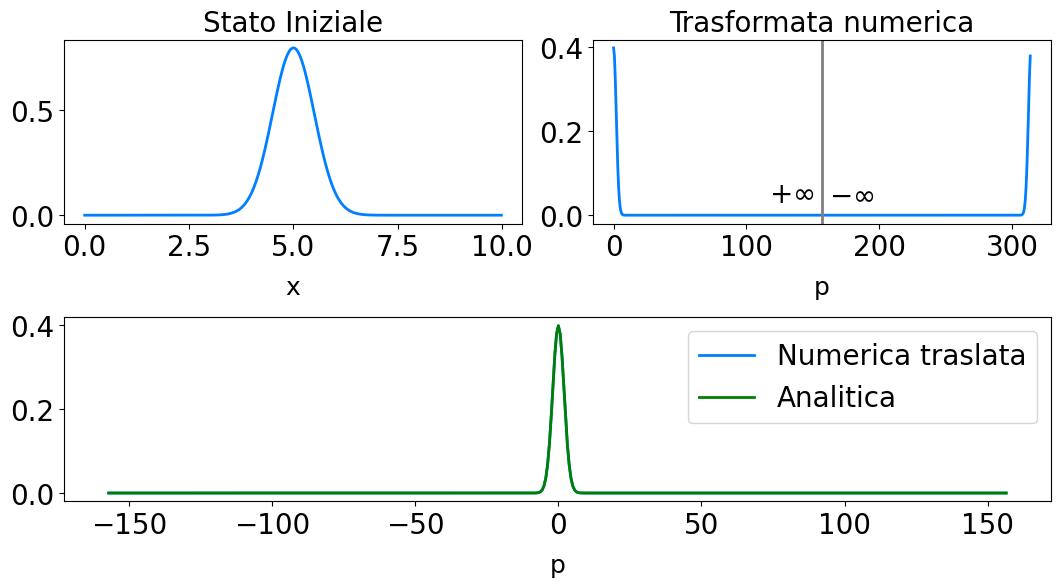
\includegraphics[width = 0.7\textwidth]{immagini/fourier.png}
    \caption{ \textcolor{dark-gray}{Modulo della trasformata di Fourier di una funzione gaussiana centrata in $x_0 = 5$. Notare come per ottenere la vera rappresentazione fisica nello spazio dei momenti sia necessario eseguire una traslazione rigida della soluzione numerica per $p >   \pi \hbar \, N / L  $}}
    \label{fig:dft_shift}
\end{figure}
Inoltre bisogna prestare attenzione al fatto che %, a causa della discretizzazione, 
la trasformata discreta mappa tutti i valori di $\tilde{\psi}(p)$ in un intervallo che non è simmetrico rispetto all'origine, come fa invece la trasformata continua. Se si considera un periodo $ 0 \le p \le 2 \pi \hbar \, N / L  $, in questo spazio sono mappati tutti i valori di $p$ da $- \infty$ a $+ \infty$, ma sono disposti in ordine inverso. Nella prima metà, tra $ 0 \le p \le \pi \hbar \, N / L  $, sono mappati i valori tra $0$ e $+ \infty$, mentre nella seconda metà, tra  $ \pi \hbar \, N / L  < p \le 2 \pi \hbar \, N / L $, sono riportati i valori corrispondenti all'intervallo tra $- \infty$ e $0$. Per costruire, quindi, la vera rappresentazione fisica della funzione d'onda nello spazio dei $p$ è necessario eseguire una traslazione rigida della $\tilde{\psi}(p)$ dall'intervallo $ \pi \hbar N / L < p \le 2 \pi \hbar \, N / L $ all'intervallo $ - \pi \hbar \, N / L  < p \le 0 $, come si può vedere dall'esempio riportato in Fig.(\ref{fig:dft_shift}).


\section{Conidizioni e vincoli sul sistema} %{Limiti e criticità}
\label{sec:limits}

I principali limiti della simulazione sono dovuti al processo di discretizzazione. 
La discretizzazione dello spazio impone ovvi limiti sulla scelta dei parametri spaziali, poiché essendo lo spazio della simulazione limitato, si perde informazione su qualsiasi oggetto definito al di fuori dell'intervallo $ 0 \le x \le L$. È quindi necessario, fare in modo che la funzione d'onda sia per lo più definita all'interno dell'intervallo, in modo tale che sia trascurabile il contributo della funzione esterno ad esso. 

La discretizzazione spaziale introduce, inoltre, due criticità dovute alla natura della trasformata discreta di Fourier. In prima istanza bisogna porre particolare attenzione alla scelta dello stato iniziale, poiché non solo è limitato lo spazio diretto, ma lo è anche lo spazio dei momenti. La discretizzazione pone dei limiti non solo sui parametri spaziali della funzione d'onda, ma anche su quei parametri capaci di modificare la forma del profilo nello spazio nei momenti. Nuovamente è necessario che tutta l'informazione nello spazio dei momenti sia contenuta nell'intervallo $ - \pi \hbar \, N / L  < p \le \pi \hbar \, N / L  $. 
Inoltre la periodicità della trasformata di Fourier genera un effetto per cui per un profilo uscente da un estremo dello spazio viene propagata l'evoluzione come entrante dall'altro estremo dello spazio. Tale effetto disturba l'evoluzione della funziona d'onda originale, rendendola scorretta. Scegliendo opportunamente i parametri, è possibile ovviare a questo problema facendo in modo che le conseguenze di questo effetto si manifestino a tempi maggiori di quelli necessari ad ottenere i risultati desiderati. 
Se, però, si volesse simulare l'andamento di un sistema per tempi lunghi è possibile ovviare a questo problema modificando la forma del potenziale agli estremi dell'intervallo. Se, infatti, si modifica $V$ in maniera tale per cui 
\begin{equation}
    V'(x) = 
        \begin{cases}
            V(x) \quad &\lambda < x < L - \lambda \\ 
             \exp \left(-i \, s\right) &\quad  \text{altrove}
        \end{cases}
    \quad \text{con} s, \lambda > 0 %\in \mathbb{R}^{+}
    \, \text{,}
    \label{eq:stp_bound}
\end{equation}
risulterà che la funzione d'onda verrà smorzata esponenzialmente ai bordi. La scelta di $s$ e $\lambda$ deve essere opportunamente valutata in modo da ottenere il risulato desiderato.

La discretizzazione temporale introduce un valore massimo possibile per il potenziale, dovuto ai termini $ \exp \left(- i V c_{j} \, \delta t\right)$, che sono funzioni periodiche per la variabile $V$. Se si immagina di far variare in maniera continua $V$, si può vedere che per $|V| > 2 \pi / \delta t \,  c_j$ si rimappano gli stessi valori dell'intervallo $0 \le |V| \le 2 \pi / \delta t \,  c_j$.
Bisogna, quindi, considerare la seguente condizione
\begin{equation}
    \underset{[0, L]}{\max} \; \abs{V(x)} < \frac{2 \pi}{\delta t \, c_{j}} \, \text{.}
    \label{eq:V_max}
\end{equation}


\chapter{Validazione del codice}
\label{ch:Validazione}

Per validare il metodo risolutivo sono stati implementati vari potenziali di cui si conosce la soluzione analitica per poter confrontare i risultati numerici con l'evoluzione esatta. In tutte le simulazioni è stata utilizzata l'eq.(\ref{eq:LT_2}) per approssimare l'operatore di evoluzione temporale, poiché tale espnsione è considerata come il miglior compromesso tra precisione e costo computazionale.

\section{Particella libera}
\label{sec:free}

\subsection{Pacchetto d'onde gaussiano}
\label{sec:WP_gaussiano}

Si ricorda la definizione di pacchetto d'onde
\begin{equation}
    \centering
    \psi(q, 0) = \frac{1}{\sqrt{2 \pi}} \int_{- \infty}^{+ \infty} dk \; g(k) \exp \left(ikq\right) \, \text{,}
    \label{eq:WP}
\end{equation}
dove $g(k)$ è la trasformata di Fourier di $\psi(q, 0)$ e porta informazione sullo stato iniziale nello spazio dei momenti. Infatti il suo modulo quadro rappresenta la probabilità che la particella abbia momento $k$.
Se si considera $g(k)$ tale per cui $|g(k)|^2$ sia gaussiana e sostituendo le definizioni
\begin{equation}
    \hbar k \equiv p - p_0 \, \text{,}   \quad q \equiv x - x_0 \, \text{,}
    \label{eq:def_kq}
\end{equation}
l'eq.(\ref{eq:WP}) si riduce alla funzione d'onda per un pacchetto gaussiano 
\begin{equation}
    \centering
    \psi(x, 0) = \left( \frac{2}{ \pi \sigma^2} \right)^{\nicefrac{1}{4}} \exp \left(-i \frac{p_{0}}{\hbar} (x -x_0)\right) \exp \left(-\frac{(x -x_0)^2}{\sigma^{2}}\right) \, \text{,}
    \label{eq:WP_gaus}
\end{equation}
dove $p_0$ rappresenta lo sfasamento del pacchetto nello spazio dei momenti ed è strettamente legato al valore dell'energia cinetica associata al pacchetto. %la grandezza che controlla l'energia cinetica associata al pacchetto $T = p_{0}^{2} / 2m$. 
In Fig.({\ref{fig:free_p_view}}) viene riportato un esempio.

\begin{figure}
    \centering
    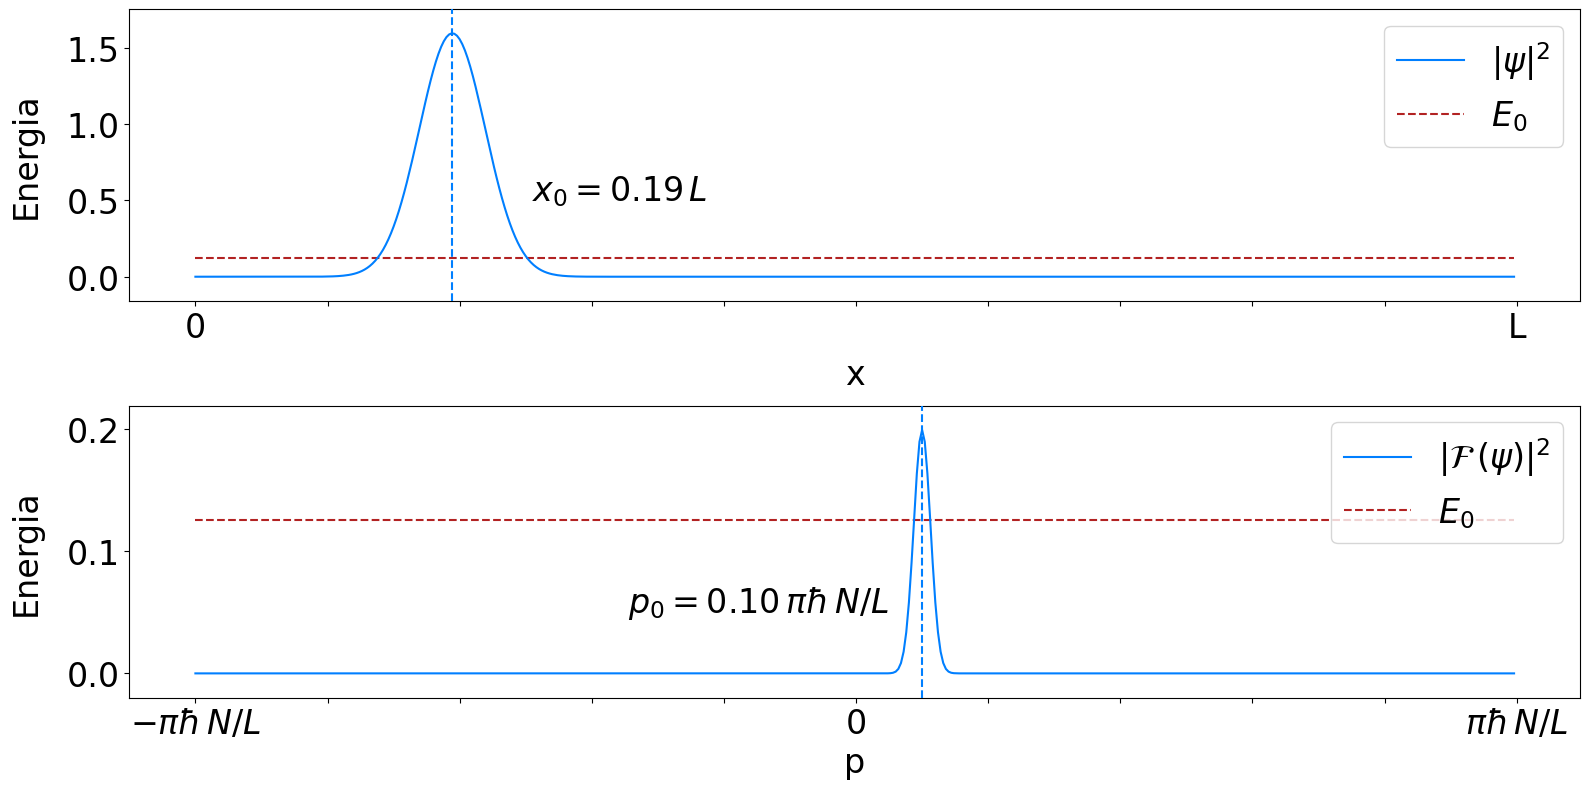
\includegraphics[width = \textwidth]{immagini/free_p_view.png}
    \caption{ \textcolor{dark-gray}{Rappresentazione dello stato inziale per un pacchetto gaussiano di onde piane, sia nello spazio diretto che nello spazio dei momenti.}}
    \label{fig:free_p_view}
\end{figure}

\subsection{Evoluzione analitica}

Con potenziale di particella libera si intende una configurazione a potenziale costante $V(x) = 0$. In tale configurazione si può considerare la soluzione analitica per l'evoluzione di un pacchetto d'onde gaussiano. 
Data l'eq.(\ref{eq:Sc_1D}), con $V(x) = 0$, questa è risolta per ogni funzione
\begin{equation}
    \centering
    \psi_{k} (x, t) = \hat{A} \exp \left[i(kx - \omega t)\right] \qquad \text{con}  \quad \omega = \frac{\hbar k^2}{2m} \, \text{.}
    \label{eq:plane_wave}
\end{equation}
Per cui è possibile costruire il pacchetto
\begin{equation}
    \centering
    \psi(q,t) = \frac{1}{\sqrt{2 \pi}} \int_{- \infty}^{+ \infty} dk \; g(k) \exp \left[i(kq - \omega t)\right] \, \text{.}
    \label{eq:WP_ev}
\end{equation}
Considerando un pacchetto gaussiano e sostituendo le definizioni nell'eq.(\ref{eq:def_kq}), si ottiene la funzione analitica per l'evoluzione libera del pacchetto nell'eq(\ref{eq:WP_gaus}) 
\begin{equation}
    \centering
    \psi(x,t) = 
    \left( \frac{2 \sigma^2}{\pi} \right)^{\nicefrac{1}{4}} 
    \left( \sigma^4 + \frac{4 \hbar^2 t^2}{m^2}   \right)^{\nicefrac{-1}{4}}
    \exp \left(i \frac{p_0}{\hbar} x\right) 
    \exp \left( - \frac{\left[ x - p_0 t / m \right]^{2}} {\sigma^2 - 2 i \hbar t / m} \right)
    e^{i \phi} \, \text{,}
    \label{eq:WP_gaus_ev}
\end{equation}
\begin{equation}
    \centering
    \text{con} \quad \phi = - \frac{1}{2} \arctan (\frac{2 \hbar t}{m \sigma_0^2}) - \frac{p_0^2}{2 m \hbar} t  \, \text{.}
\end{equation}
In Fig.(\ref{fig:free_ev}) si riporta il confronto tra la soluzione numerica e quella analitica per alcuni tempi successivi.

\begin{figure}
    \centering
    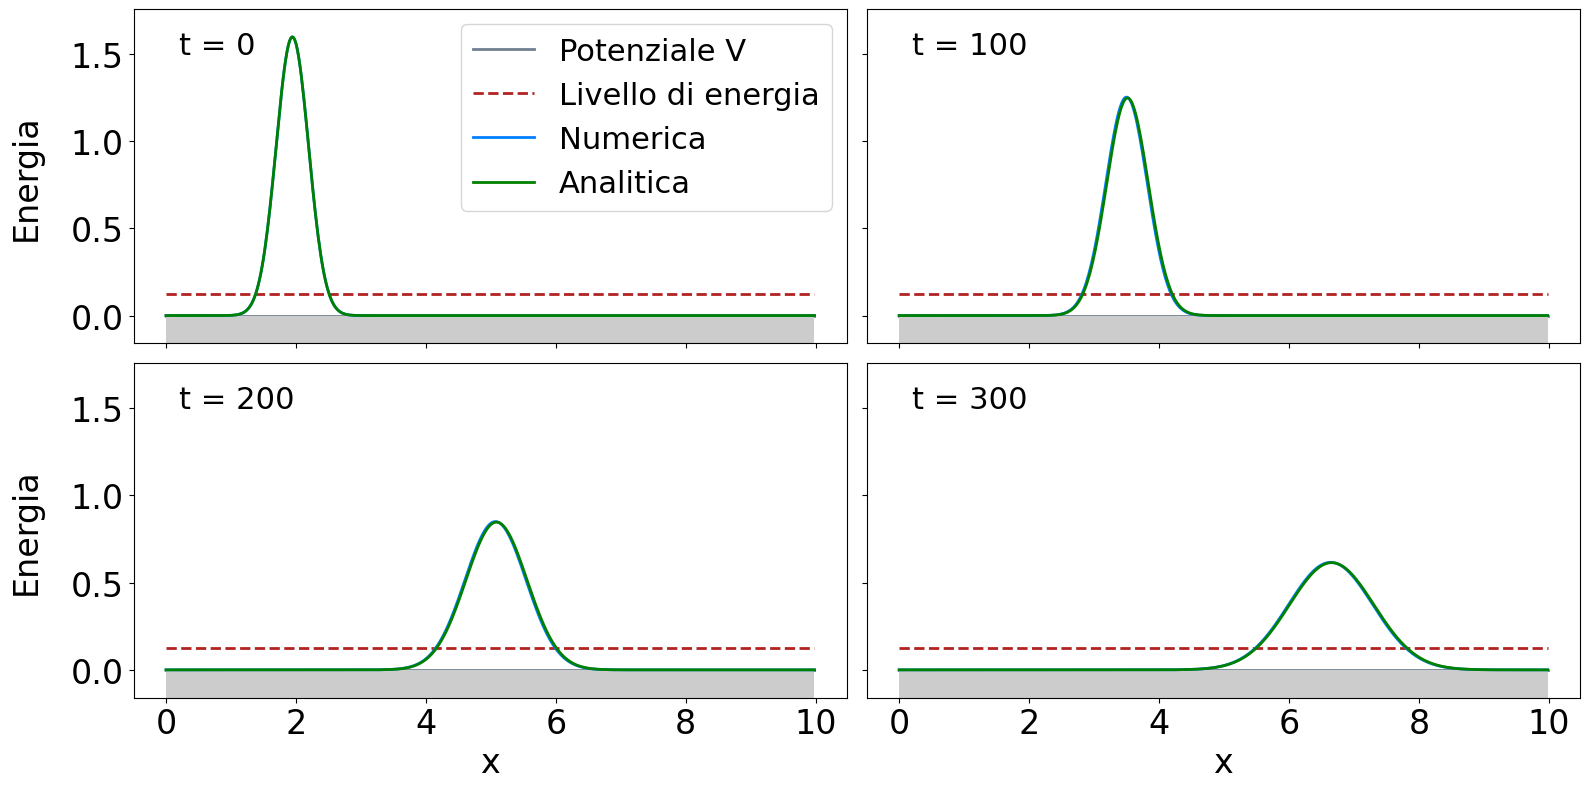
\includegraphics[width = \textwidth]{immagini/free_ev.png}
    \caption{ \textcolor{dark-gray}{Confronto tra soluzione numerica e soluzione analitica per una particella libera. Si può notare un'ottima sovrapposizione tra le due.}}
    \label{fig:free_ev}
\end{figure}


\section{Oscillatore armonico}
\label{sec:arm}

Si ricordano definizione di potenziale armonico
\begin{equation}
    \centering
    V(x) = \frac{1}{2} m \omega^2 (x -x_0)^2
\end{equation}
e i principali risultati ottenuti dalla soluzione dell'equazione di Schr\"odinger stazionaria
\begin{equation}
    \centering
    E_k = (\frac{1}{2} + k) \hbar \omega \, \text{,} \qquad \psi_{k} = \left( \frac{\beta^2}{\pi} \right)^{\nicefrac{1}{4}} \frac{1}{\sqrt{2^{k} \, k!}} \exp \left(-\frac{\beta^2 x^2}{2}\right) H_{k}(\beta x) \, \text{,}
    \label{eq:arm_res}
\end{equation}
\begin{equation}
    \centering
    \text{con}  \quad k \in \mathbb{N} \text{ ,  } \beta = \sqrt{\frac{m \omega}{\hbar}} \, \text{.}
\end{equation}
È noto che se si considera l'eq.(\ref{eq:U}) per gli stati stazionari questa si riduce a 
\begin{equation}
    \centering
    \psi_{k}(x, t) = \exp \left( - \frac{i}{\hbar} E_k t \right) \psi_{k} (x,0)      \, \text{.}
    \label{eq:ev_eigenstate}
\end{equation}
Dato che è sempre possibile scrivere un generico stato iniziale come combinazione lineare di autostati si trova che l'evoluto temporale risulta essere
\begin{equation}
    \centering
    \psi(x, t) = \sum_{k} c_{k} \, \exp \left( - \frac{i}{\hbar} E_k t \right) \psi_k (x,0) \qquad \text{con} \quad\psi(x,0) = \sum_{k} c_{k} \,  \psi_k (x,0)        \, \text{,}
    \label{eq:ev_combinazione}
\end{equation}
che è la soluzione esatta del problema.

In Fig.(\ref{fig:superpos}) si riporta il confronto tra la soluzione numerica e l'evoluzione analitica per la sovrapposizione di auotostati dell'oscillatore armonico
\begin{equation}
    \centering
    \psi(x, 0) = \frac{1}{\sqrt{2}} \left( \ket{0} + \ket{1} \right)   \, \text{.}
    \label{eq:superpos}
\end{equation}

\begin{figure}
    \centering
    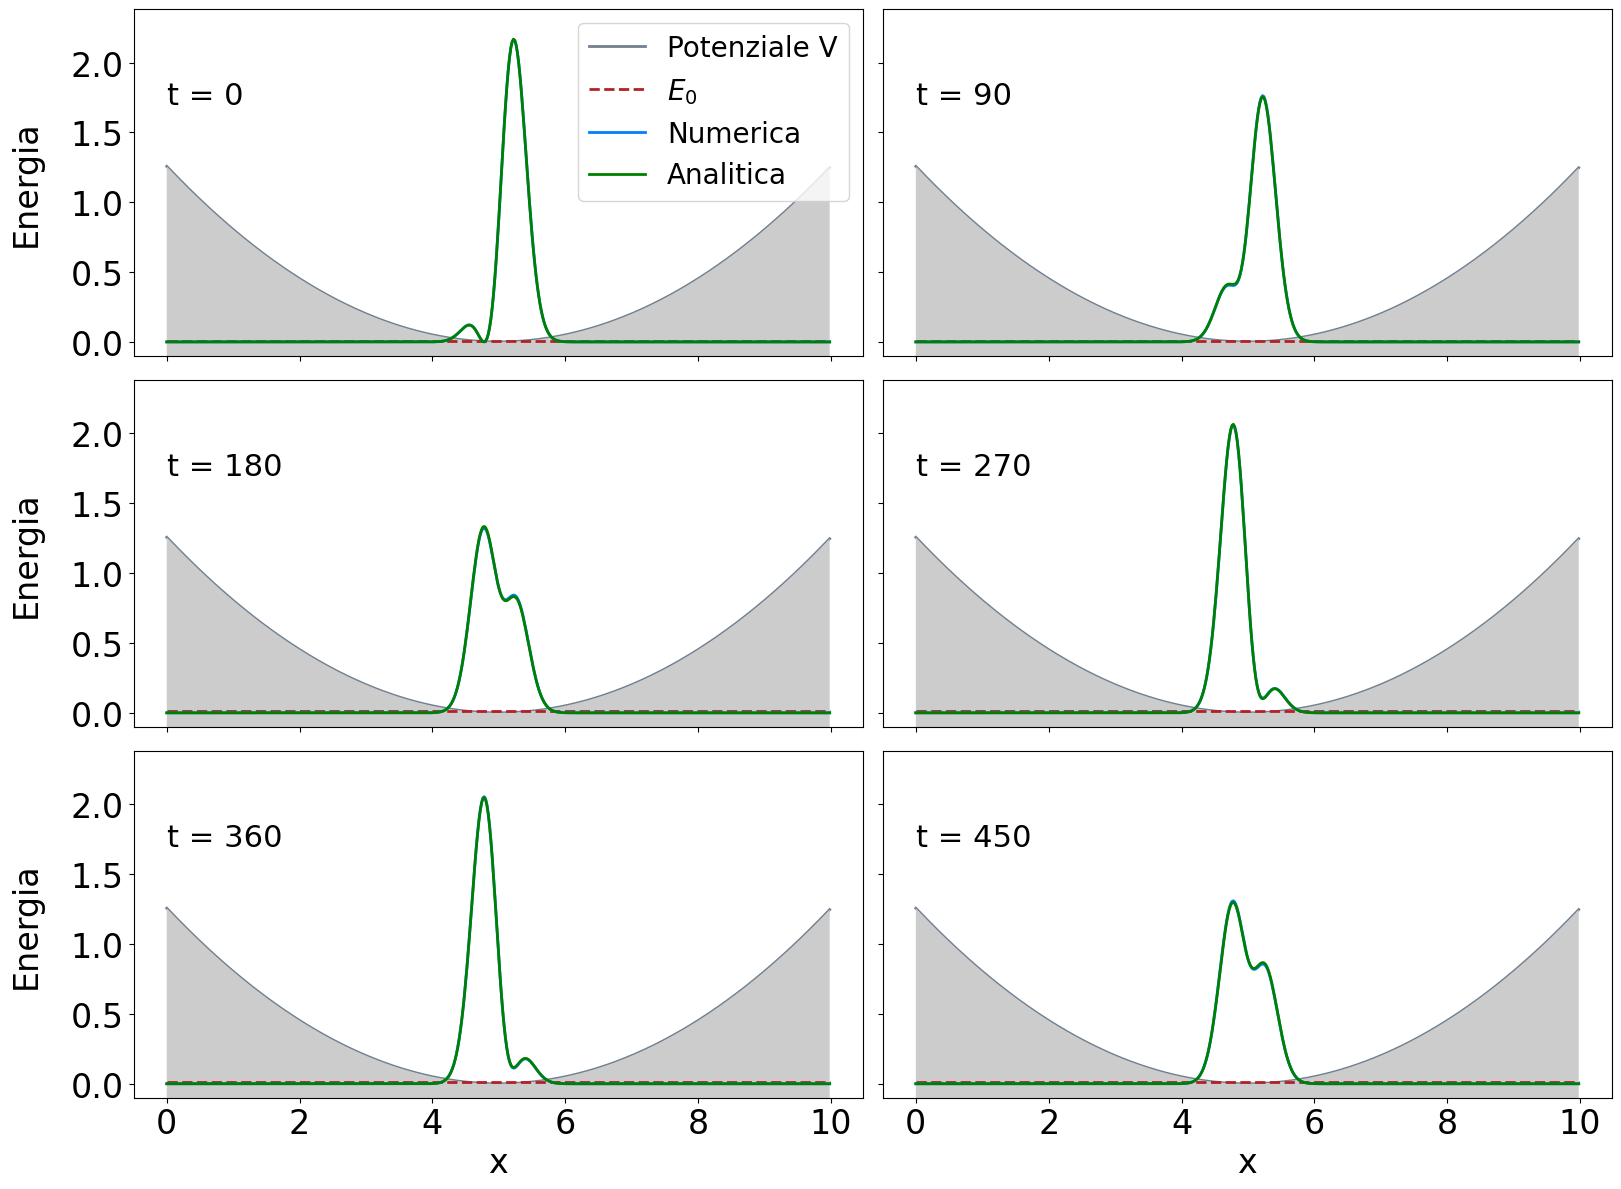
\includegraphics[width = \textwidth]{immagini/superposition.png}
    \caption{ \textcolor{dark-gray}{Confronto tra soluzione numerica e soluzione analitica per la sovrapposizione di autostati nell'eq.(\ref{eq:superpos}).}}
    \label{fig:superpos}
\end{figure}


\section{Stati coerenti}
\label{sec:coherent}

Con stati coerenti \cite{CT:QM} si intendono gli autostati dell'operatore di distruzione dell'oscillatore armonico. Sono divenuti celebri, poiché vennero utilizzati da Schr\"odinger come dimostrazione del principio di corrispondenza. Tali stati, infatti, sono caratterizzati da una dinamica molto simile al comportamento oscillatorio di un oscillatore armonico classico. 
Infatti l'evoluzione analitica per il modulo quadro di uno stato coerente, $|\psi_{\alpha}(x, t)|^{2}$, corrisponde ad una traslazione rigida di una gaussiana con 
\begin{equation}
    \centering
    \expval{x}_{t} = \hat{A} \, \cos (\theta - \omega t) \, \text{,} \quad
    \expval{p}_{t} = m \omega \hat{A} \, \sin (\theta - \omega t) \qquad
    \text{dove} \quad \hat{A} = \sqrt{\frac{2 \hbar}{m \omega}} \,|\alpha| \, \text{.}
    \label{eq:coherent_an}
\end{equation}
Queste equazioni per i valori medi corrispondono alle soluzioni classiche dell'oscillatore armonico.

Gli stati coerenti sono definiti tramite una sovrapposizione infinita, del tipo nell'eq.(\ref{eq:ev_combinazione}), di autostati di oscillatore armonico nel seguente modo
\begin{equation}
    \centering
    \ket{\alpha} = \exp \left(- \frac{|\alpha|^2}{2}\right) \sum_{k=0}^{+ \infty} \left( \frac{\alpha^k}{k!} \right) \ket{k} \, \text{.}
    \label{eq:def_coherent}
\end{equation} 
Nelle simulazioni numeriche non è possibile estendere la somma a $+\infty$, per questo è necessario troncarla ad un valore finito.

In Fig.(\ref{fig:coherent_ev}) si riporta il confronto tra la soluzione analitica e numerica per l'evoluzione di uno stato coerente. Lo stato iniziale è costruito tramite la formula nell'eq.(\ref{eq:def_coherent}), dove la sommatoria è stata troncata a 170 \footnote{La scelta di questo numero è dovuta al fatto che, in Python, il numero più alto possibile per cui il suo fattoriale si possa assegnare ad una variabile di tipo float è 170.}. Mentre nella sezione (\ref{sec:Wp_arm}) si studia l'evoluzione di pacchetto gaussiano di onde piane anche in confronto ad uno stato coerente.

\begin{figure}
    \centering
    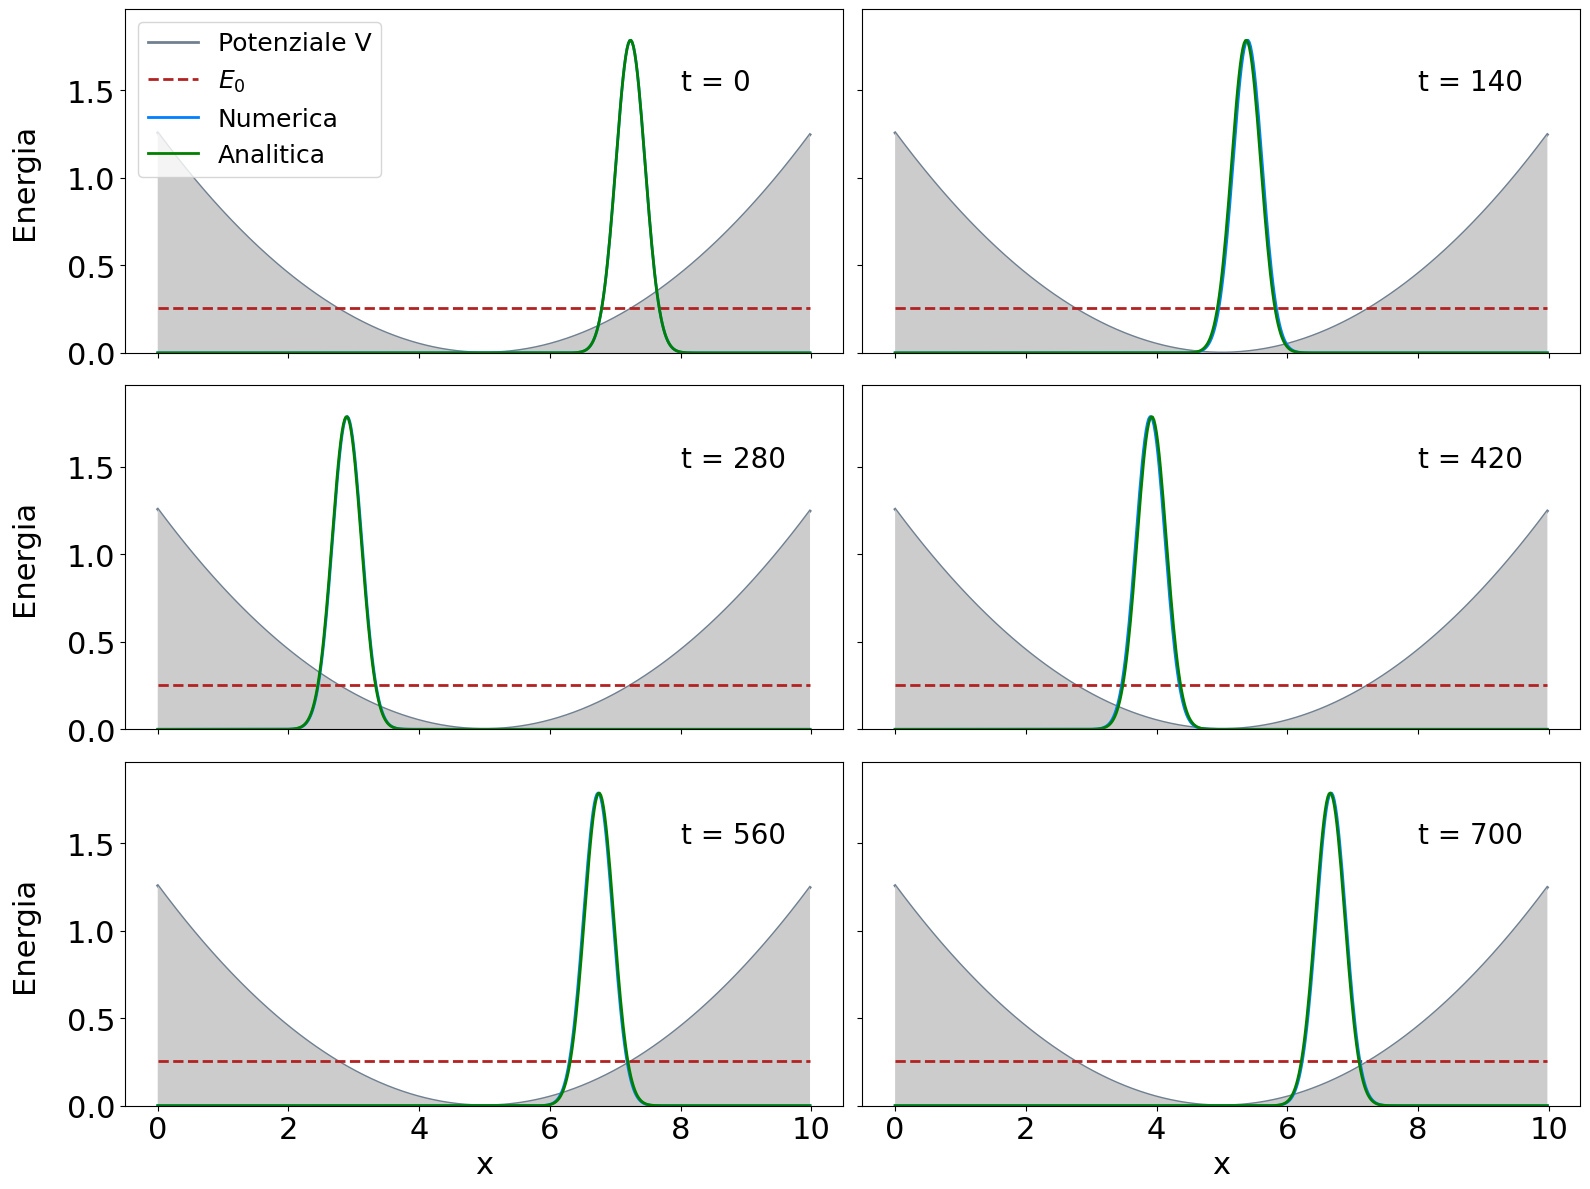
\includegraphics[width = \textwidth]{immagini/coherent_ev.png}
    \caption{ \textcolor{dark-gray}{Confronto tra soluzione numerica e soluzione analitica per uno stato coerente. Si noti come le dimensioni caratteristiche della funzione gaussiana $|\psi_{\alpha}(x, t)|^{2}$ non vengano deformate durante l'evoluzione.}}
    \label{fig:coherent_ev}
\end{figure}



\section{Potenziale di P\"oschl-Teller}
\label{sec:RL}

Il potenziale di P\"oschl-Teller (PT), applicato nel contesto della meccanica quantistica, prende la forma 
\begin{equation}
    \centering
    V(x) = -\frac{\hbar^2 \alpha^2}{2m} \frac{\nu (\nu + 1)}{\cosh^2 (\alpha x)} \quad \text{con} \nu \in \mathbb{N} \, \text{.}
    \label{eq:pot_PT}
\end{equation}
Questo potenziale è di particolare importanza poiché si può dimostare che $\forall \nu$ il coefficiente di trasmissione, $T$, per una funzione d'onda incidente sul potenziale risulta essere pari a $1$. Per questo gli viene attribuito l'aggettivo \textsl{reflectionless}.   
Come per il potenziale armonico è possibile risolvere l'equazione agli autovalori per PT
\begin{equation}
    \centering
    \left[ - \frac{\hbar^{2}}{2m} \, \frac{d^2}{dx^2} -\frac{\hbar^2 \alpha^2}{2m} \frac{\nu (\nu + 1)}{\cosh^2 (\alpha x)}  \right] \, \psi_k (x, t) = E_k \, \psi_k (x, t) \, \text{.}
    \label{eq:einge_eq_PT}
\end{equation}
Con le opportune sostituzioni è possibile rendere l'equazione adimensionale
\begin{equation}
    \centering
    \hat{H_{\nu}} \psi_k (\xi, t) =  \left[ \hat{P}^2 - \frac{\nu (\nu + 1)}{\cosh^2 (\xi)}  \right] \, \psi_k (\xi, t) = k^2 \, \psi_k (\xi, t) \, \text{,} 
    \label{eq:PT_adim}
\end{equation}
\begin{equation}
    \text{con  } \hat{P} = -i \frac{d}{d \xi}
\end{equation}
e definire gli operatori di innalzamento e abbassamento
\begin{equation}
    \centering
    a_{\nu} = \hat{P} - i \nu \tanh(\hat{\xi}) \; \text{,} \quad  a_{\nu}^{\dagger} = \hat{P} + i \nu \tanh(\hat{\xi}) \; \text{.}
\end{equation}
Sfruttando questi operatori è possibile calcolare la forma esplicita per lo stato di \textsl{ground} risolvendo 
\begin{equation}
    \centering
    \left[-i \frac{d}{d \xi} - i \nu \tanh(\xi) \right] \psi_{0, \nu} (\xi) = 0
\end{equation}
e dimostrare che $H_{\nu}$ e $H_{\nu - 1}$ condividono lo stesso spettro a meno dello stato di \textsl{ground} $\ket{0}_{\nu}$.
Per $\nu = 0$ si ottiene l'equazione di particella libera, si può quindi legare i noti autostati di $\hat{H_0}$ a quelli di $\hat{H_1}$ tramite
\begin{equation}
    \ket{k}_1 = a_{1}^{\dagger} \ket{k}_0
    \label{eq:autostati_eq}
\end{equation}
e trovare la forma analitica degli autostati dello spettro continuo. Il procedeimento si può estendere per ricorsione ad ogni valore di $\nu$ \cite{Jaffe:RL_sol}.

Conoscendo l'espressione esplicita della base di autostati è possibile risolvere il problema scomponendo lo stato iniziale sulla base in analogia con quanto fatto in precedenza.
Con $\nu = 1$, dall'eq.(\ref{eq:autostati_eq}) si ottengono gli autostati e autovalori
\begin{equation}
    \centering
    \psi_{k}(x) = \left[ \frac{i k - \alpha \, \tanh (\alpha x)}{ik + \alpha}\right] \exp(ikx)  \; \text{,} \quad E_k = \frac{\hbar^2 k^2}{2 m } \quad \text{con} \; k \in \mathbb{R} \, \text{,}
\end{equation}
che generano uno spettro continuo e infinito. Si può, dunque, costruire un pacchetto d'onde di autostati 
\begin{equation}
    \centering
    \psi(x, t) = \frac{1}{\sqrt{2 \pi}} \int_{-\infty}^{+\infty} dk \, A(k) \, \psi_{k}(x) \exp \left(- \frac{i}{\hbar} E_k t \right) \, \text{,}
    \label{eq:WP_RL_def}
\end{equation}
con $\hbar k \equiv p - p_0$.
Fissando $A(k) = (ik + \alpha) \phi_0(k)$, dove $\phi_0(k)$ è la trasformata di Fourier di un pacchetto gaussiano (vedere l'eq.(\ref{eq:WP_gaus})) e risolvendo l'integrale, si ottiene la soluzione per l'evoluzione di un pacchetto d'onde gaussiano di autostati di PT  
\begin{align}
    \centering
    \psi(x, t) &= N \left[i \frac{p_0}{\hbar} - \frac{x - x_0 - v_{g}t}{ \sigma_0 s_t} - \alpha \tanh (\alpha x) \right] \psi_{G}(x,t)    \, \text{,} \\
    s_t &= \frac{\sigma_0}{2} \left(1 + i \frac{2 \hbar t}{ m \sigma_0^2} \right) \, \text{,} 
    \label{eq:WP_RL_ev}
\end{align}
con $\psi_{G}(x,t)$ la funzione d'onda dell'evoluzione libera di un pacchetto gaussiano di onde piane di eq.(\ref{eq:WP_ev}) e $v_g = p_0 / m$ è la velocità di gruppo\cite{Mousavi:PT_WP}.

In Fig.(\ref{fig:WP_RL}) si riporta il confronto tra la soluzione numerica e la soluzione analitica e si trova un ottimo accordo tra le due.

\begin{figure}
    \centering
    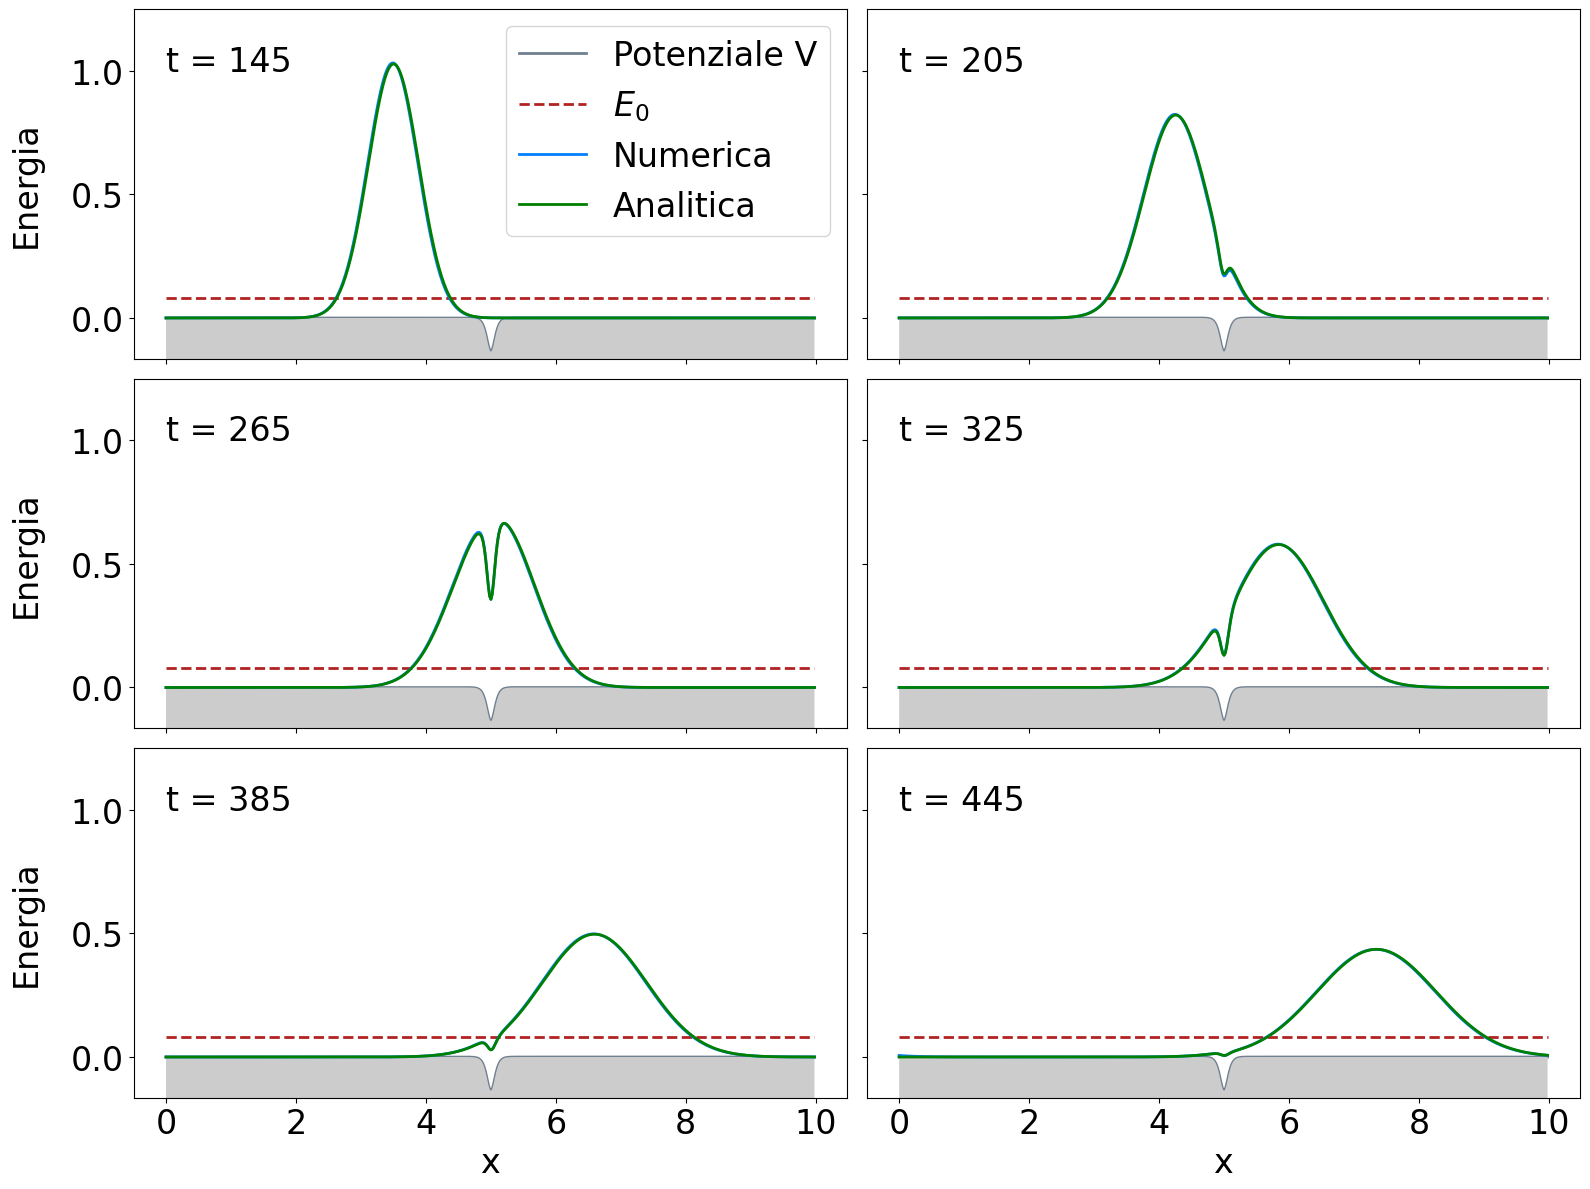
\includegraphics[width = \textwidth]{immagini/WP_RL.png}
    \caption{ \textcolor{dark-gray}{Confronto tra soluzione numerica e soluzione analitica per un pacchetto gaussiano di autostati di PT. Si trova un ottimo accordo tra la simulazione numerica e l'evoluzione esatta.}}
    \label{fig:WP_RL}
\end{figure}

\chapter{Applicazioni}
\label{ch:applicazioni}

L'utente tramite l'interfaccia grafica ha la possibilità di scegliere tra alcuni potenziali pre-impostati:
\begin{itemize}[nolistsep]
    \item particella libera,
    \item oscillatore armonico,
    \item buca e barriera finita di potenziale,
    \item gradino di potenziale,
    \item barriera coulombiana semplificata,
    \item potenziale \textsl{reflectionless} di P\"oschl-Teller,
\end{itemize}
Da combinare con i seguenti stati iniziali:
\begin{itemize}[nolistsep]
    \item pacchetto gaussiano di onde piane, 
    \item autostati dell'oscillatore armonico e loro sovrapposizioni,
    \item stati coerenti,
    \item pacchetto gaussiano di autostati del potenziale di PT.
\end{itemize}
In questa sezione non solo si riportano alcuni dei risultati ottenuti partendo dagli stati sopracitati, ma anche altre soluzioni di particolare interesse.


\section{Buca finita di potenziale}
\label{sec:finite_hole}

La buca finita è definita da
\begin{equation}
    \centering
    V(x) =
    \begin{cases}
        \; -V_0  \quad &\text{per  } a \le x \le b  \\
        \; 0 \qquad &\text{altrove}      
    \end{cases} 
    \quad \text{con  } V_0 > 0 \, \text{.}
\end{equation}
La soluzione di questo problema permette di mettere in evidenza un fenomeno caratteristico della meccanica quantistica: la riflessione di una particella può avvenire anche in corrispondenza di una diminuzione dell'energia potenziale. 
%ben riassunto nella frase di David Jeffrey Griffiths: \textcolor{red}{\dots \dots \dots}
Un tale comportamento non è riscontrabile nella meccanica classica. Secondo le equazioni di Newton $m \ddot{\vec{x}} = -\nabla V(\vec{x}, t)$, per cui risulta che, in corrispondenza di una buca di potenziale, la particella subisca una determinata accelerazione nella direzione del moto dovuta alla prima discontinuità e successiva decelerazione in corrispondeza della seconda. In meccanica quantistica questo non è certo che accada, come mostrato in Fig.(\ref{fig:finite_hole}): infatti esiste una probabilità diversa zero che la particella si trovi nella zona antecedente la buca con momento opposto.

\begin{figure}
    \centering
    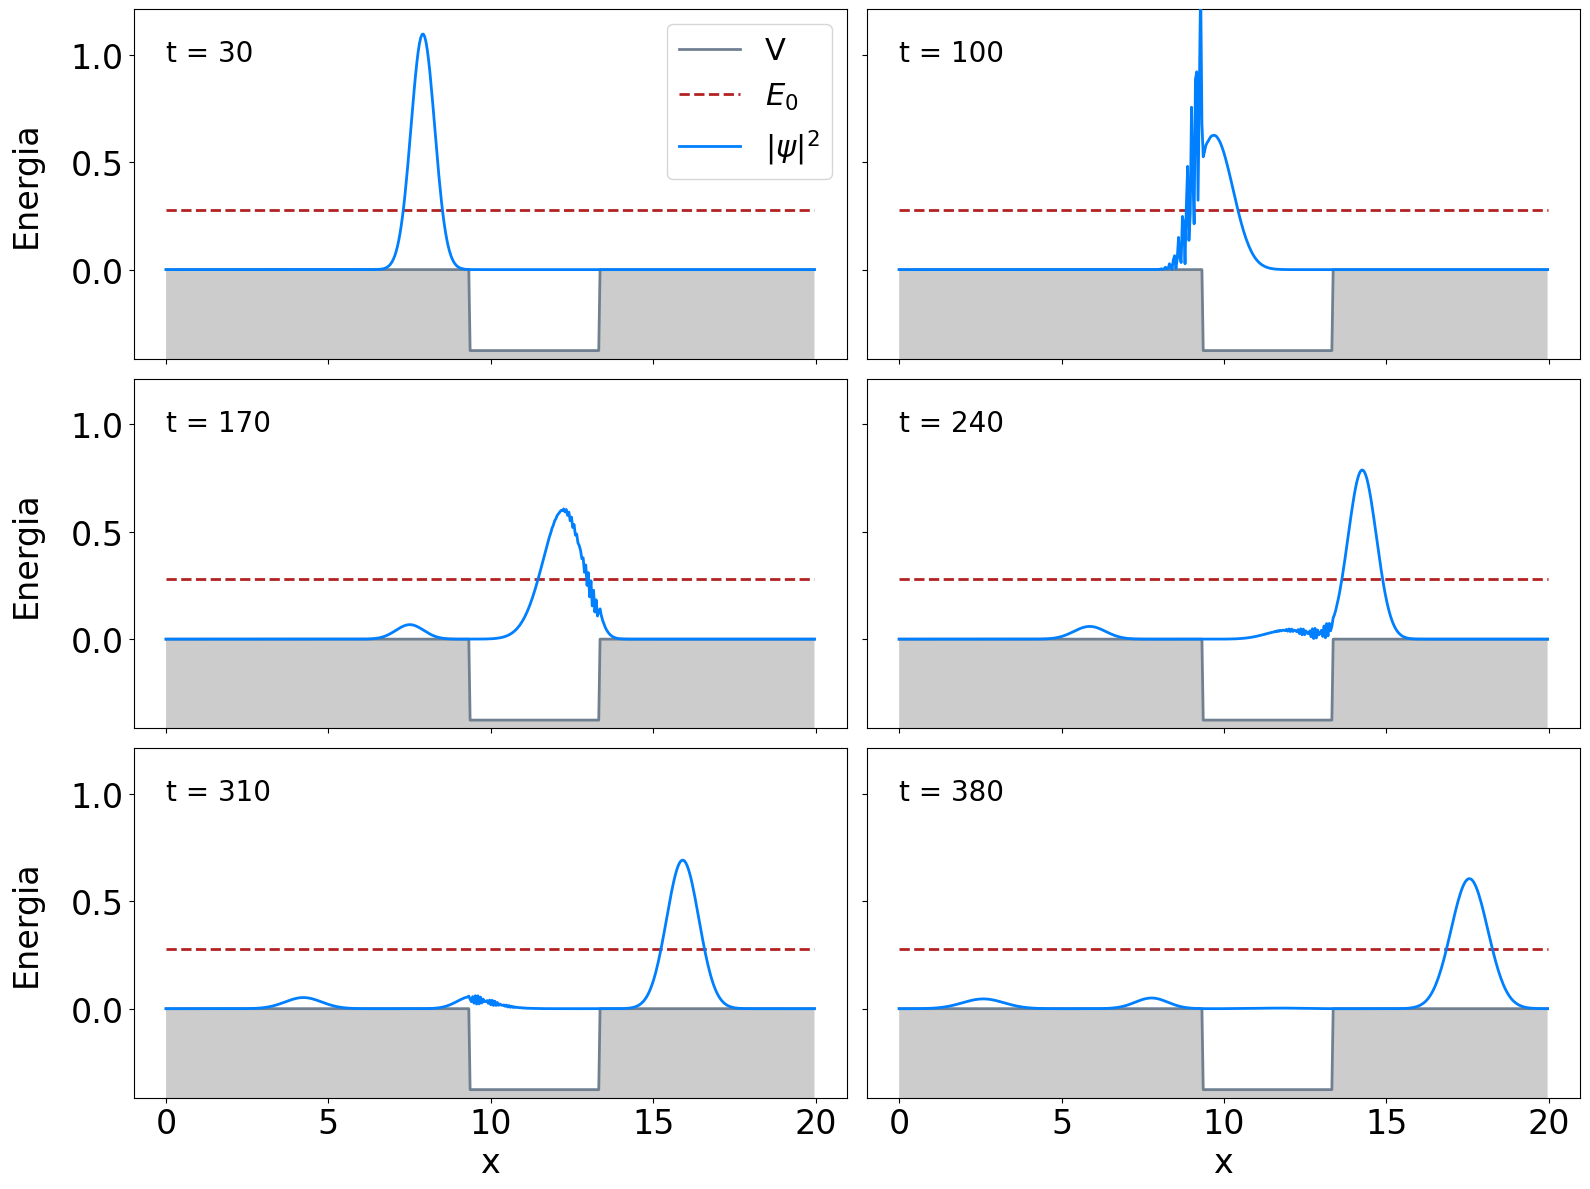
\includegraphics[width = \textwidth]{immagini/hole.png}
    \caption{ \textcolor{dark-gray}{Evoluzione di un pacchetto gaussiano di onde piane che interagisce con una buca finita di potenziale. Si noti il fatto che parte dell'onda viene riflessa.}}
    \label{fig:finite_hole}
\end{figure}

\section{Barriera coulombiana semplificata}
\label{sec:coulomb}

Nel codice è stato implementato un potenziale
\begin{equation}
    \centering
    V(x) = 
    \begin{cases}
        \, 0 \quad &\text{per} \quad x \le \tilde{x} \\
        \, \left( x - \tilde{x} + (1 / \, V_0)\right)^{-1} \quad &\text{per} \quad x > \tilde{x} 
    \end{cases}
    \qquad \text{con  } V_0 > 0 \, \text{,}
    \label{eq:tunnel}
\end{equation} 
per mettere in evidenza un altro fenomeno caratteristico della meccanica quantistica: l'effetto tunnel.
Fenomeno attraverso il quale si può spiegare l'emissione di particelle $\alpha$ dai nuclei, durante i decadimenti. Infatti si è scelto questo potenziale perché ricorda la forma del potenziale che risentono le particelle all'interno nuclei.
In Fig.(\ref{fig:tunnel}) si può vedere che, nonostante la particella non abbia l'energia sufficiente ad oltrepassare la barriera, una parte della funzione d'onda viene trasmessa. In Fig.(\ref{fig:RT_tunnel}) sono stati calcolati i coefficienti di riflessione e di trasmissione.

\begin{figure}
    \centering
    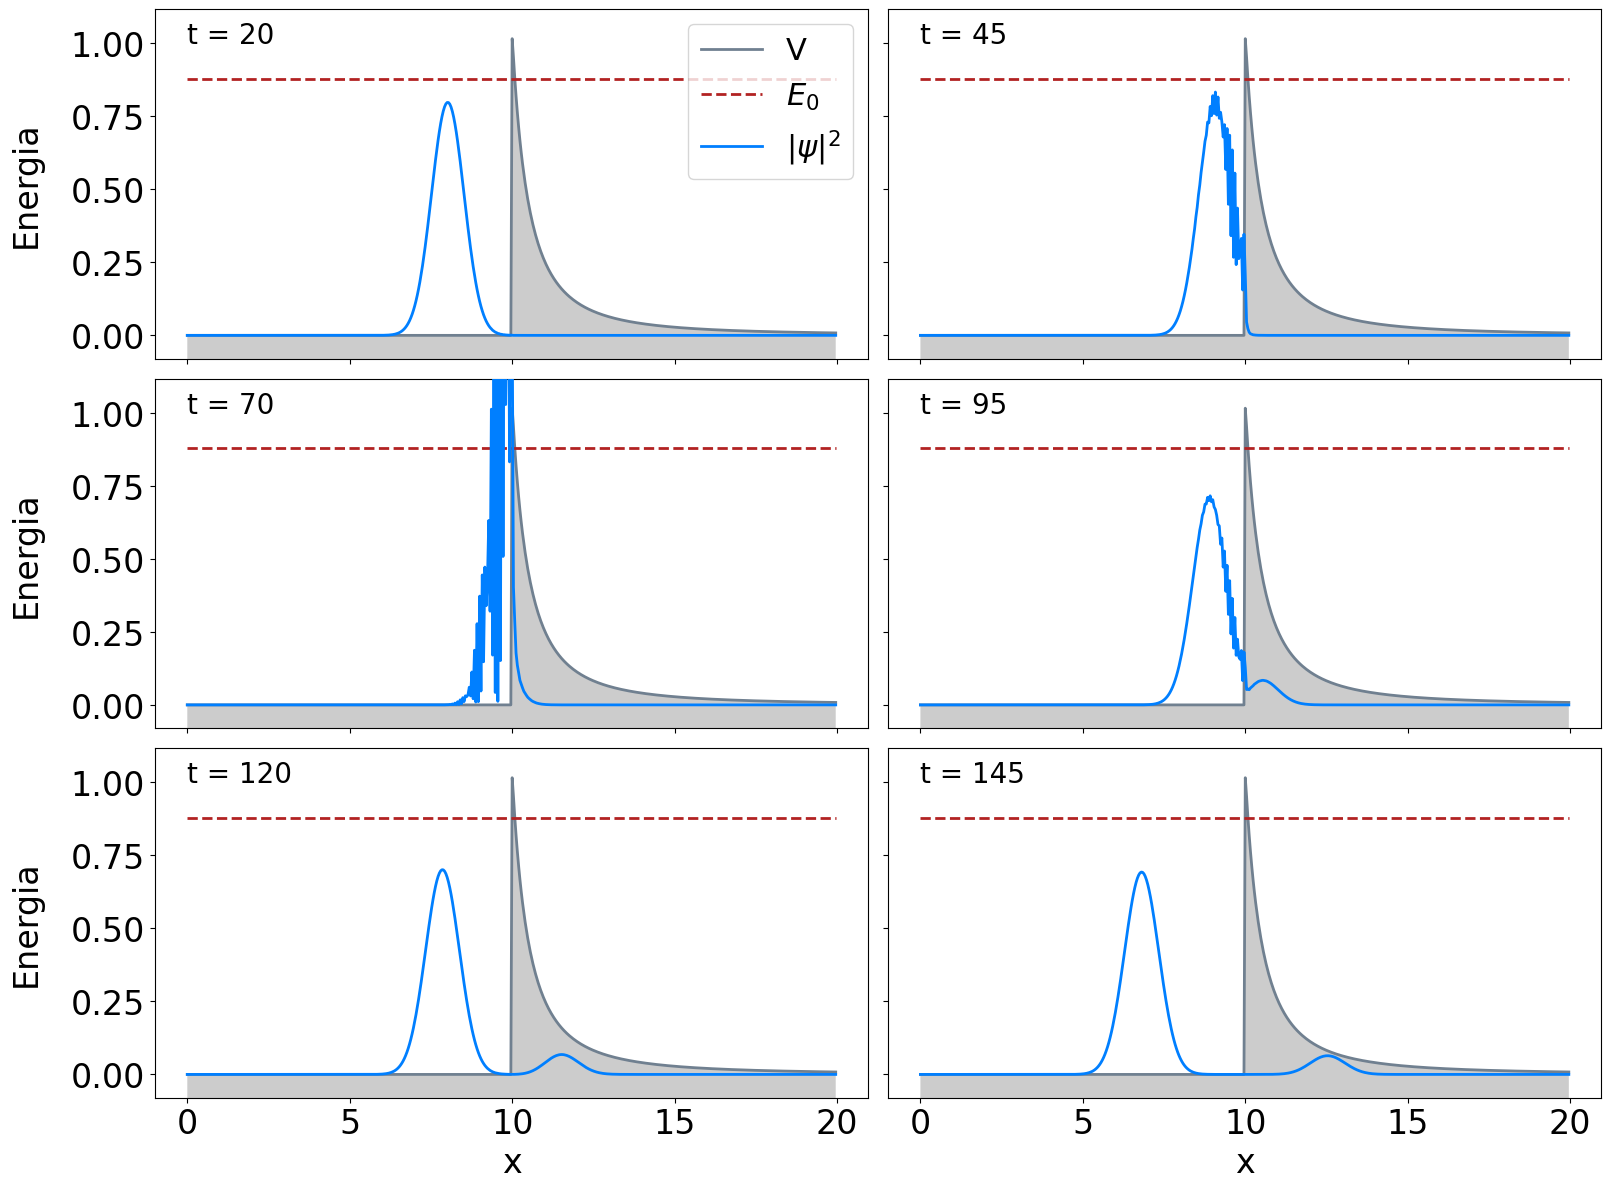
\includegraphics[width = \textwidth]{immagini/tunnel.png}
    \caption{ \textcolor{dark-gray}{Visualizzazione grafica dell'effetto tunnel per con potenziale dato dall'eq.(\ref{eq:tunnel}).}}
    \label{fig:tunnel}
\end{figure}
\begin{figure}
    \centering
    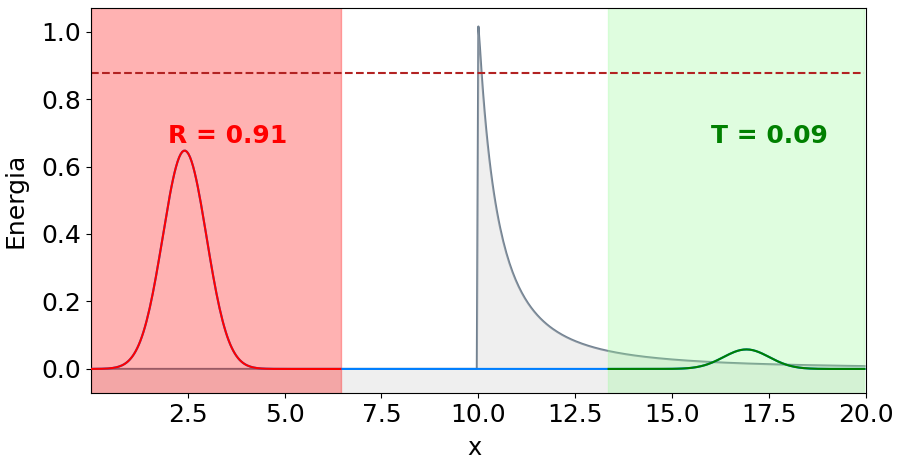
\includegraphics[width = 0.7\textwidth]{immagini/RT_tunnel.png}
    \caption{ \textcolor{dark-gray}{Coefficienti di riflessione e trasmissione calcolati per la simulazione in Fig.(\ref{fig:tunnel}). %con $t = 145$. 
    }}
    \label{fig:RT_tunnel}
\end{figure}



\section{Pacchetto gaussiano in potenziale armonico}
\label{sec:Wp_arm}

In questa viene eseguito un confronto tra l'evoluzione di uno stato coerente e l'evoluzione di un pacchetto gaussiano di onde piane a cui è associata la stessa energia.
Come si può vedere in Fig.(\ref{fig:co_vs_WP}), la dinamica del valore medio $\expval{x}_g$ del pacchetto gaussiano si %del centro di massa
sovrappone alla dinamica del valore medio $\expval{x}_c$ dello stato coerente. Per cui si può affermare che la dinamica di $\expval{x}_g$ sia facilmente interpretabile anche tramite la meccanica classica. D'altra parte mentre gli stati coerenti mantegono le dimensioni del profilo gaussiano, il pacchetto di onde piane subisce continue defomazioni lungo il moto. Emerge un comportamento puramente quantistico per cui la varianza del pacchetto subisce delle contrazioni e delle dilatazioni periodiche di periodo pari alla metà di quello dell'oscillatore armonico classico\cite{Tsuru:gaus_harmonic}.    

\begin{figure}
    \centering
    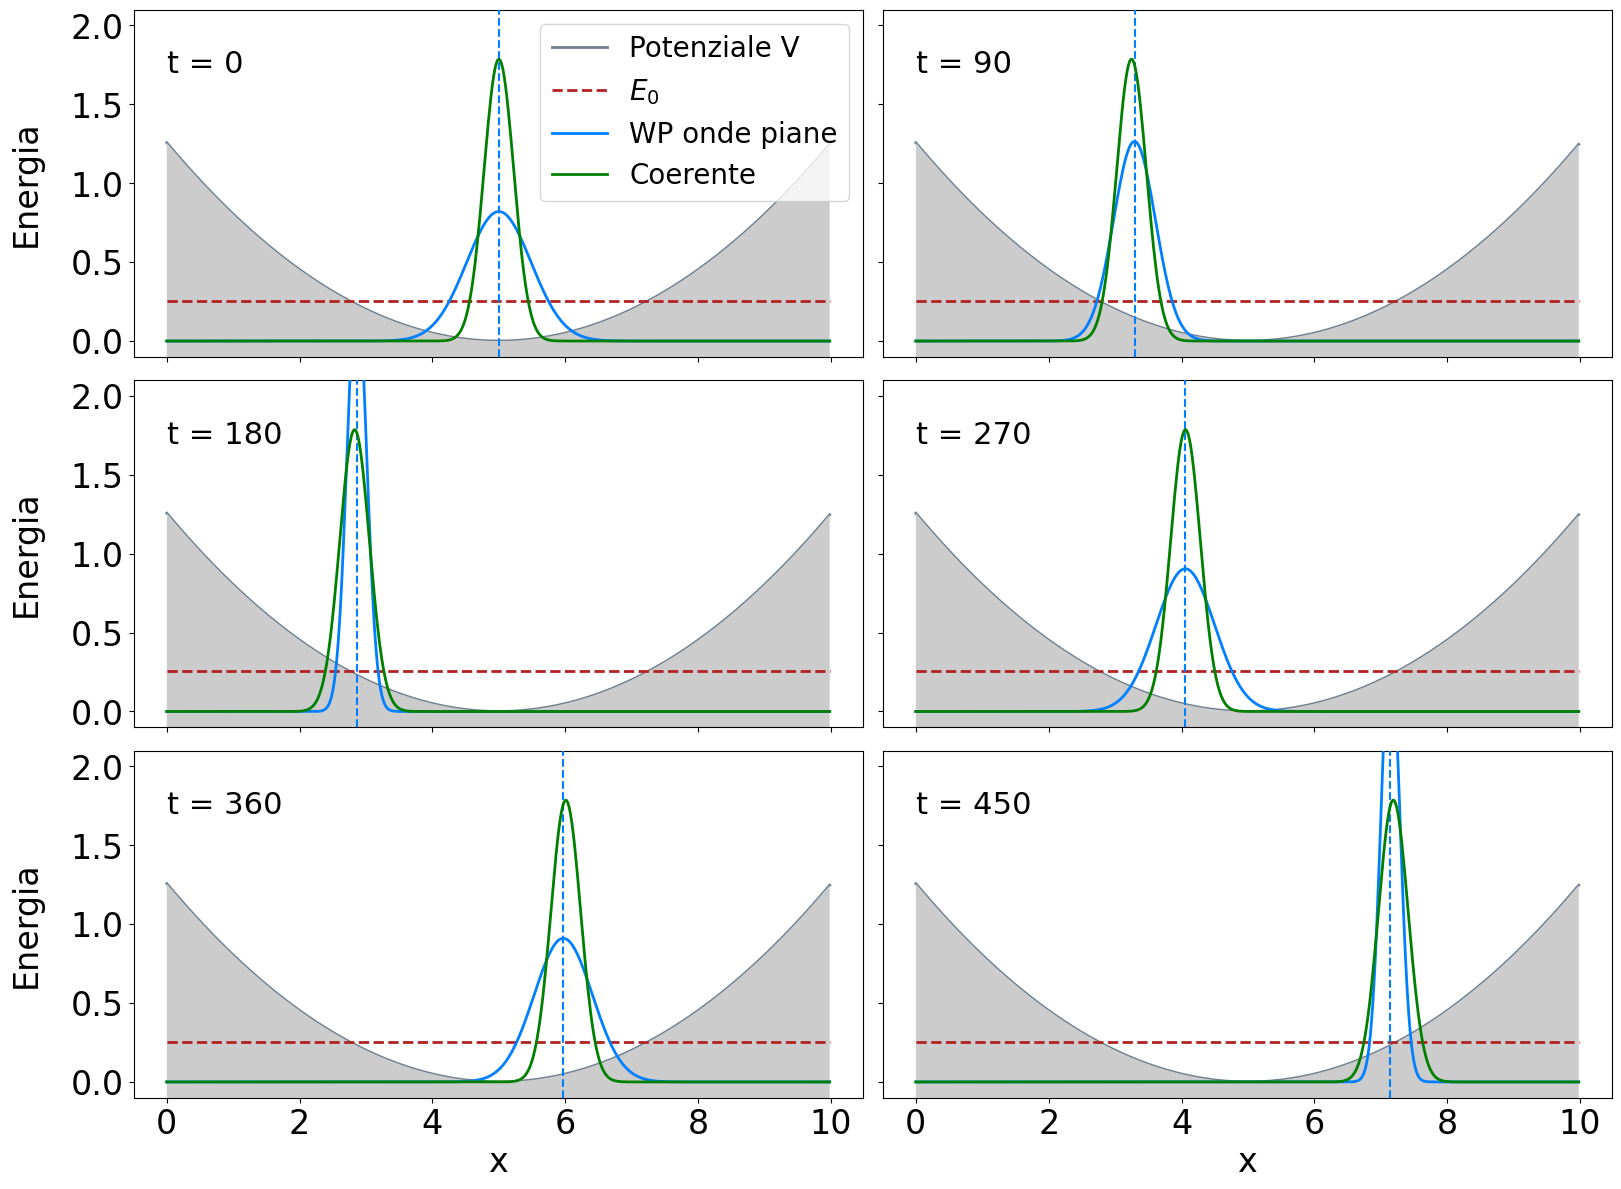
\includegraphics[width = \textwidth]{immagini/coherent_vs_WP.png}
    \caption{ \textcolor{dark-gray}{Confronto tra l'evoluzione di uno stato coerente e un pacchetto gaussiano di onde piane.}}
    \label{fig:co_vs_WP}
\end{figure}

\section{Pacchetto gaussiano nel potenziale di P\"oschl-Teller}
\label{sec:Wp_PT}

Se si considera un pacchetto gaussiano soggetto al potenziale di P\"oschl-Teller, risulterà che questo verrà interamente trasmesso, come sottolineato nella sezione (\ref{sec:RL}).
Si può studiare la deformazione subita dal pacchetto durante il moto e confrontarla con un pacchetto di autostati di PT e l'evoluzione libera, come in Fig.(\ref{fig:PT_conf}).
Il pacchetto trasmesso continua ad essere un pacchetto di forma gaussiana, ma ci sono due importanti differenze rispetto all'evoluzione libera: il valore medio $\expval{x}_g$, rappresentato in grafico tramite le linee verticali, del pacchetto trasmesso risulta precedere il valore medio $\expval{x}_l$ del pacchetto libero. Inoltre la varianza del primo risulta essere inferiore rispetto alla varianza del secondo\cite{Lecker:RL}. In confronto al pacchetto di autostati risulta che il pacchetto gaussiano risenta in maniera meno importante gli effetti del potenziale, è infatti preceduto dal pacchetto di autostati e ha un varianza maggiore\cite{Mousavi:PT_WP}.

\begin{figure}
    \centering
    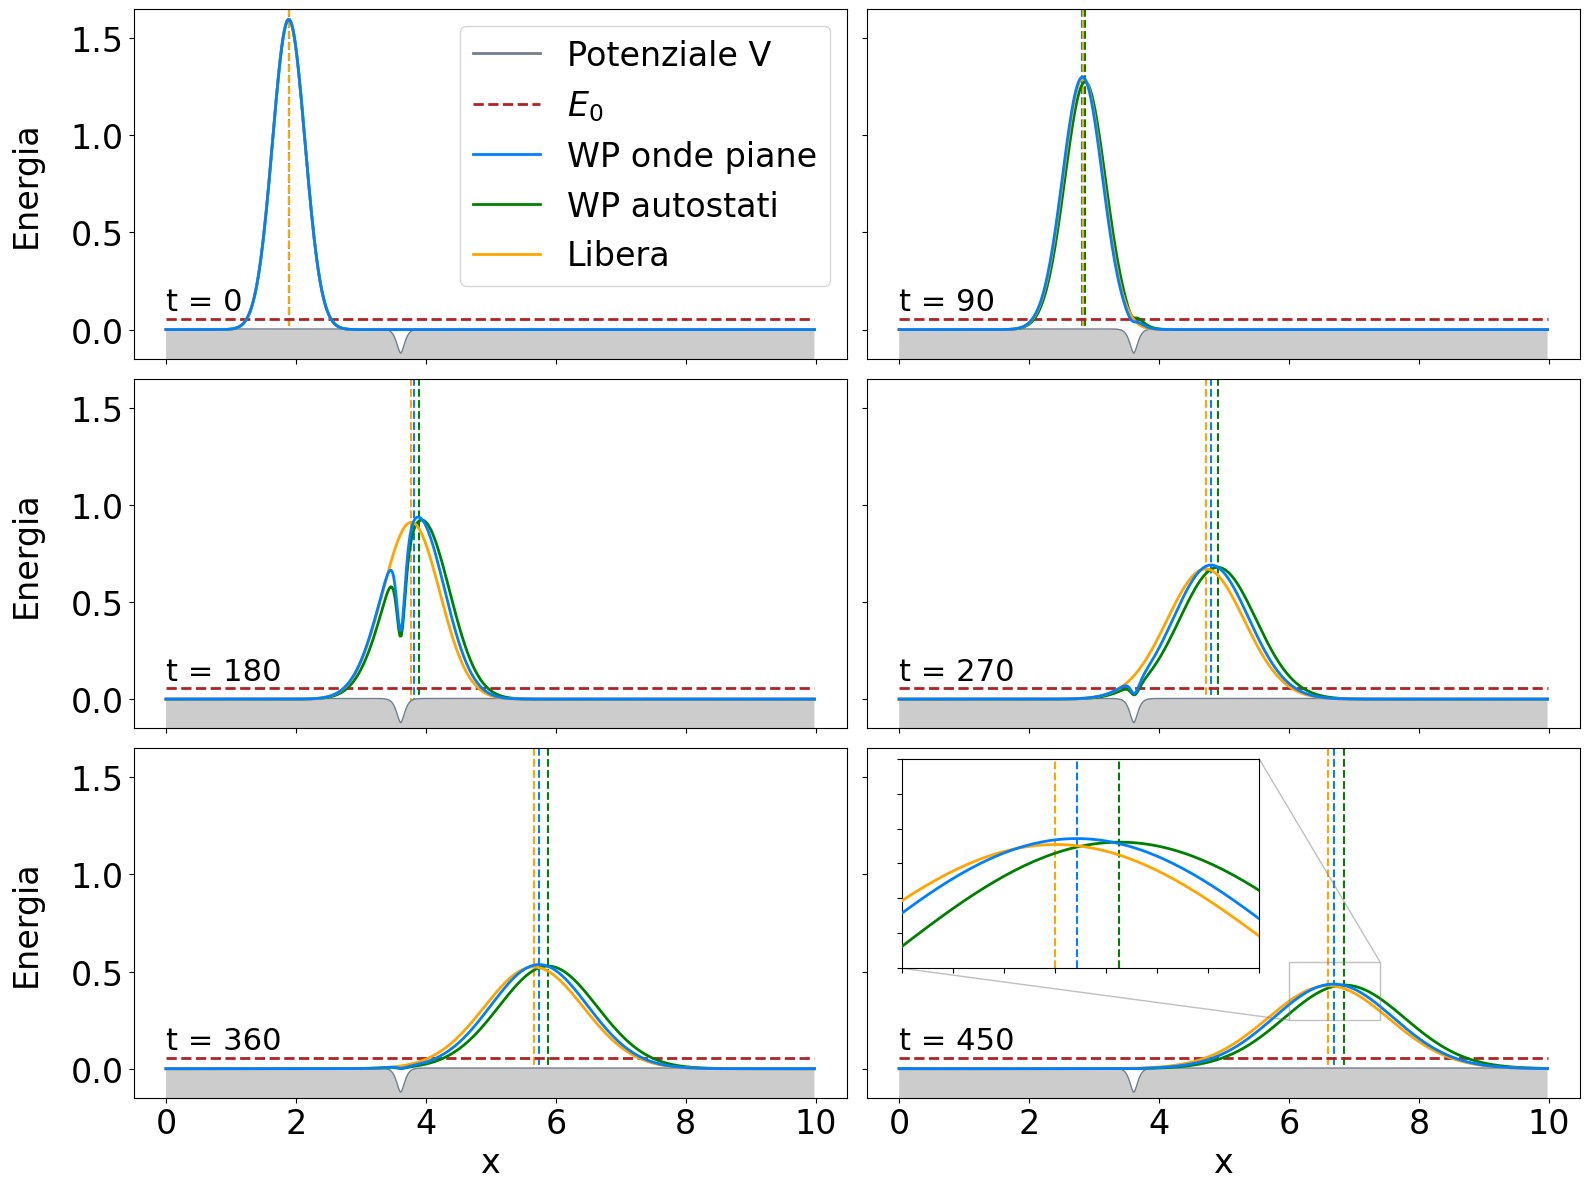
\includegraphics[width = \textwidth]{immagini/PT_num.png}
    \caption{ \textcolor{dark-gray}{Confronto tra l'evoluzione di un pacchetto gaussiano di onde piane libero (arancione) e soggetto al potenziale PT (azzurro). In verde si riporta l'evoluzione per un pacchetto gaussiano di autostati di PT.}}
    \label{fig:PT_conf}
\end{figure}


\section{Potenziale dipendente dal tempo}
\label{sec:t_dep}

Come anticipato è possibile risolvere anche problemi con potenziale dipendente dal tempo.
Come esempio si è scelto di implemenatare il potenziale 
\begin{equation}
   \centering
   V(x, t) = \alpha \, (x-x_0)^2 +  \frac{| \sin (\omega  \, t) |} {1 + \beta \, (x-x_0)^2}
\end{equation}
dove $\alpha$, $\beta$ e $\omega$ sono dei parametri reali positivi.
Come si può vedere in Fig.(\ref{fig:t-dep}) è evidente come la funzione d'onda reagisca al potenziale mentre questo cambia forma.

\begin{figure}
   \centering
    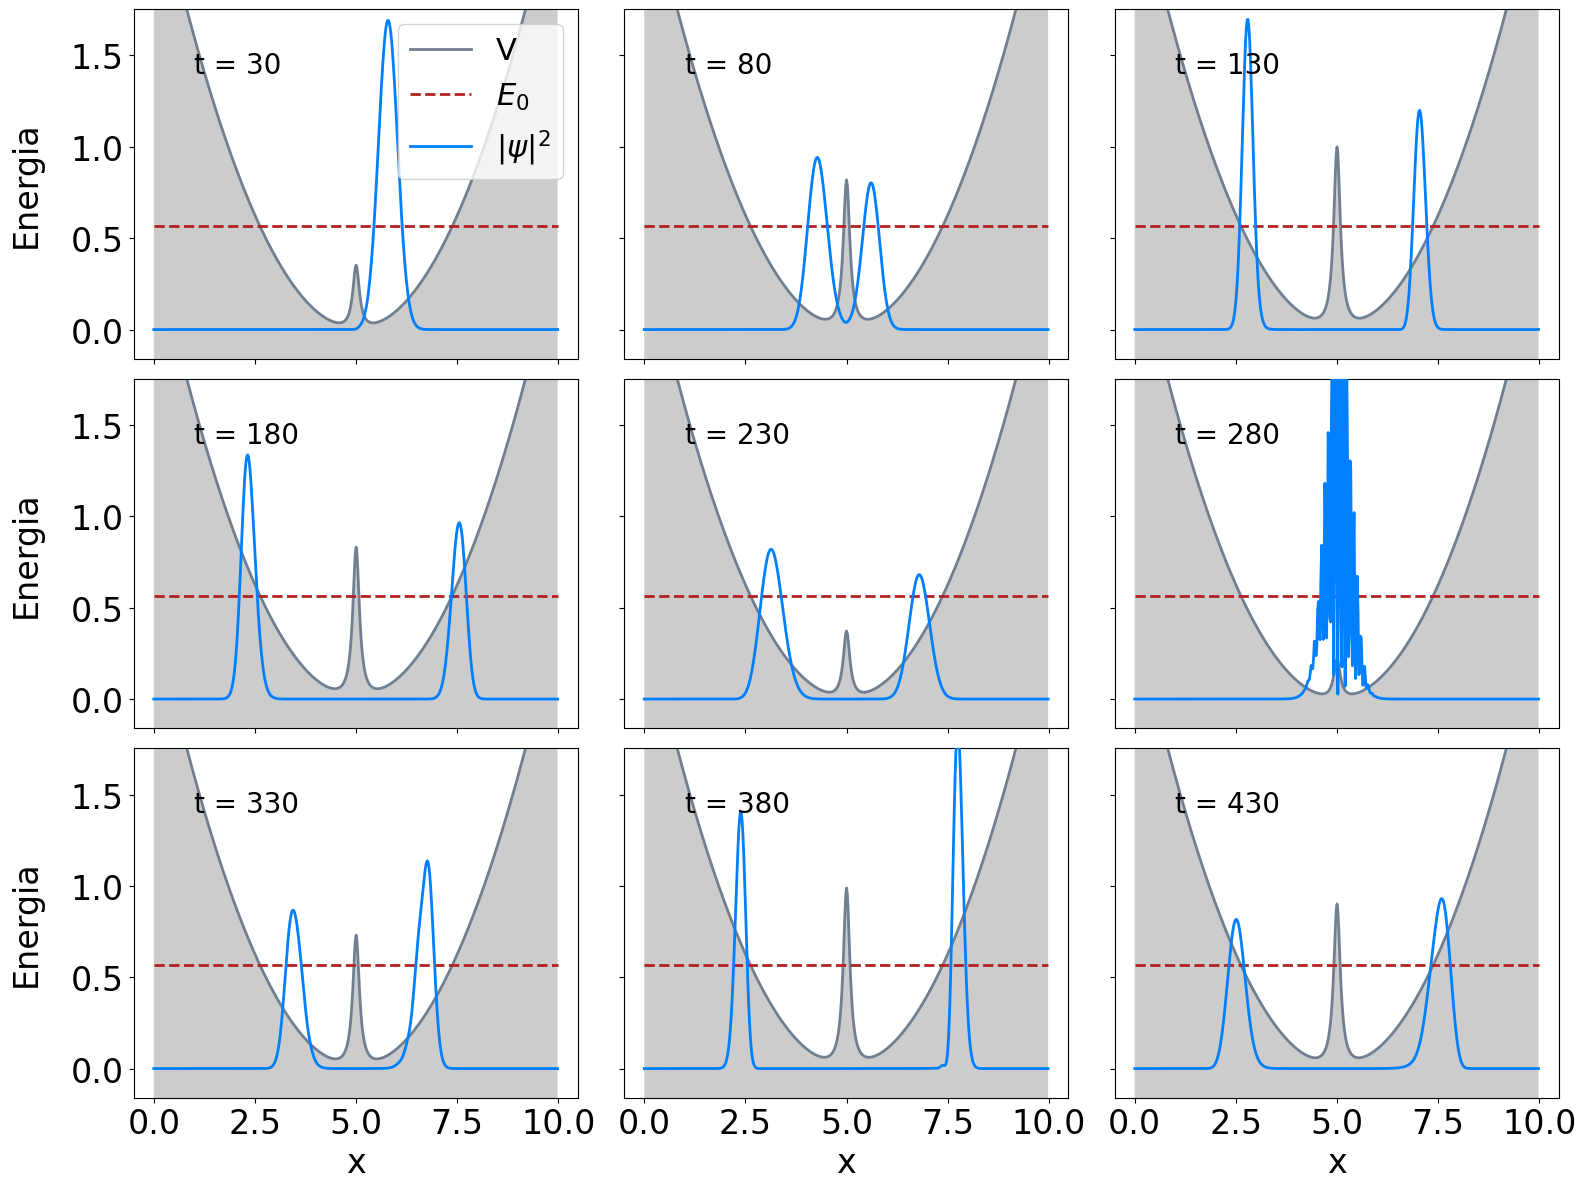
\includegraphics[width = \textwidth]{immagini/t-dep.png}
    \caption{ \textcolor{dark-gray}{Evoluzione di un pacchetto gaussiano di onde piano che interagisce con un potenziale dipendente dal tempo. Notare come per $t \, \approx \, 80$ la funzione d'onda venga separata tra le due regioni per poi sovrapporsi nuovamente per  $t \, \approx \, 280$. Il parametro t rappresenta il numero di volte in cui è stato applicata la funzione di evoluzione. }}
    \label{fig:t-dep}
\end{figure}

\chapter{Barriera infinita}
\label{ch:inf}

Come riportato nella sezione \ref{sec:limits}, non è possibile definire potenziali che non rispettino l'eq.(\ref{eq:V_max}). Il caso particolare della barriera infinita 
\begin{equation}
    V(x) = 
    \begin{cases}
        0 \quad &\text{per} \quad x < \tilde{x} \\
        \infty \quad &\text{per} \quad x \geq \tilde{x} \; \text{,}
    \end{cases}
    \label{eq:pot_inf}
\end{equation}
è però risolvibile lasciando evolvere un pacchetto opportunamente costruito in un potenziale costante $V = 0$. La presenza di una barriera infinita si traduce matematicamente nell'equazione
\begin{equation}
    \psi(\tilde{x}, t) = 0 \quad \forall t \; \text{,}
    \label{eq:cond_dir}
\end{equation}
nota anche come condizione al bordo di Dirichlet. 
Se si considera la funzione d'onda antisimmetrica rispetto a $\tilde{x}$ di $\psi(x,t)$, costruita con
\begin{equation}
    \psi_{\text{A}}(x -\tilde{x}, t) =  - \psi(\tilde{x} - x , t) \; \text{,} 
\end{equation}    
questa, in un potenziale libero, evolverà in direzione opposta rispetto a $\psi$. Nel momento in cui si considera la sovrapposizione dei due, $\Psi(x,t) = \psi(x, t) + \psi_{\text{A}}(x, t)$, si ottiene per costruzione che l'eq.(\ref{eq:cond_dir}) è identicamente verificata $\forall t$. 
La soluzione del problema proposto risulta essere $\Psi(x,t)$ valutata nel'intervallo $(-\infty, 0 \, ]$. In Fig.(\ref{fig:inf}) si riportano i risultati di una simulazione numerica per un pacchetto gaussiano in un potenziale di eq.(\ref{eq:pot_inf}), risolto con il metodo appena descritto.

\begin{figure}
    \centering
    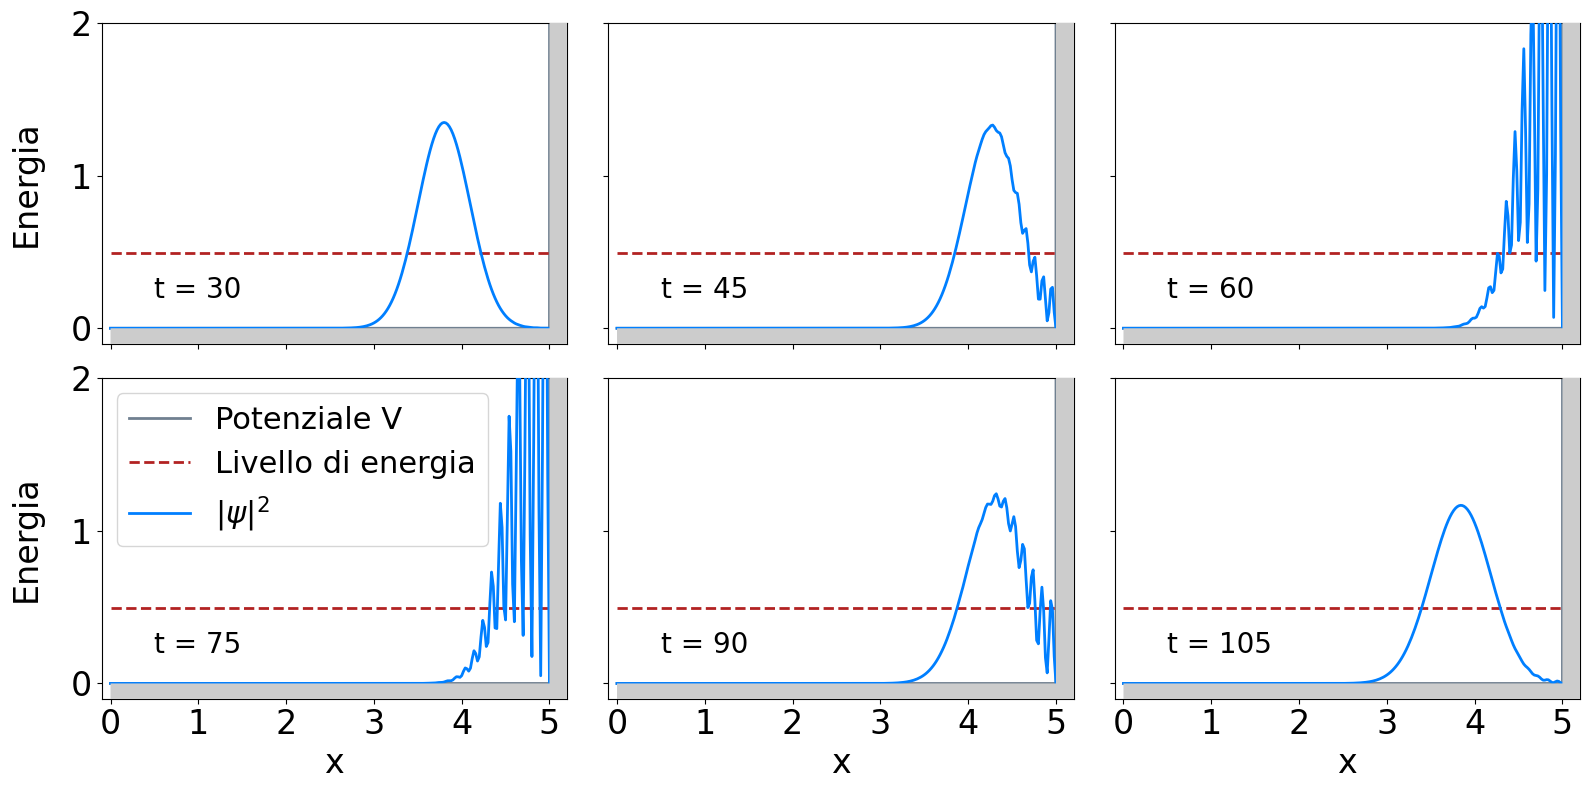
\includegraphics[width = \textwidth]{immagini/inf.png}
    \caption{ \textcolor{dark-gray}{Evoluzione di un pacchetto gaussiano di onde piano che interagisce con una barriera di potenziale infinita. }}
    \label{fig:inf}
\end{figure}

\chapter{Descrizione software}
\label{ch:interface}

Nel seguente capitolo si entra nel dettaglio di come sia stato strutturato e scritto il codice e inoltre si descrive la procedura di utilizzo delle varie componenti. 

Il software è diviso in tre componenti principali:
\begin{enumerate} [nolistsep]
    \item un interfaccia grafica dove l'utente ha la possibilità di gestire i parametri iniziali,
    \item l'algorirmo di simulazione,
    \item alcuni strumenti grafici per la visualizzazione dei risultati.
\end{enumerate}
Ognuna di queste componenti è indipendente dalle altre, poiché le informazioni sono passate attraverso file che vengono ogni volta aggiornati. In questo modo è sempre possibile risalire ai parametri utilizzati, modificarli senza usare l'ambiente grafico e gestire tutto da riga di comando.
In Fig.(\ref{fig:schema}) è riassunto lo schema di funzionamento. Si crea, tramite l'interfaccia, un file \textsl{Par.py} che riassume tutti i parametri iniziali. Si lancia la simulazione dall'interfaccia e l'algoritmo simulativo salva i risultati in una cartella precedentemente selezionata. I risultati sono poi animati tramite un altro strumento grafico. Si noti che, da riga di comando, è possibile lanciare in maniera indipendente sia l'algoritmo simulativo sia gli strumenti di animazione, purché siano presenti i file intermedi necessari.

Il codice è stato scritto utilizzando il linguaggio Python appoggiandosi alle librerie esterne:
\begin{itemize}[nolistsep]
    \item Numpy, per le funzioni matematiche e la gestione dei vettori,
    \item Matplotlib, per generare i grafici e le animazioni,
    \item Tkinter, per la costruzione dell'interfaccia grafica,
    \item Numba, per compilare le funzioni di evoluzione temporale.
\end{itemize}
Attraverso gli strumenti grafici è possibile, oltre che visualizzare i risultati sotto forma di animazione, confrontare le soluzioni numeriche con le soluzioni analitiche e stimare l'errore, visualizzare l'evoluzione in contemporanea nello spazio diretto e nello spazio dei momenti, calcolare i coefficienti di riflessione e di trasmissione e i valori medi associati alla funzione d'onda.

\begin{figure}
    \centering
    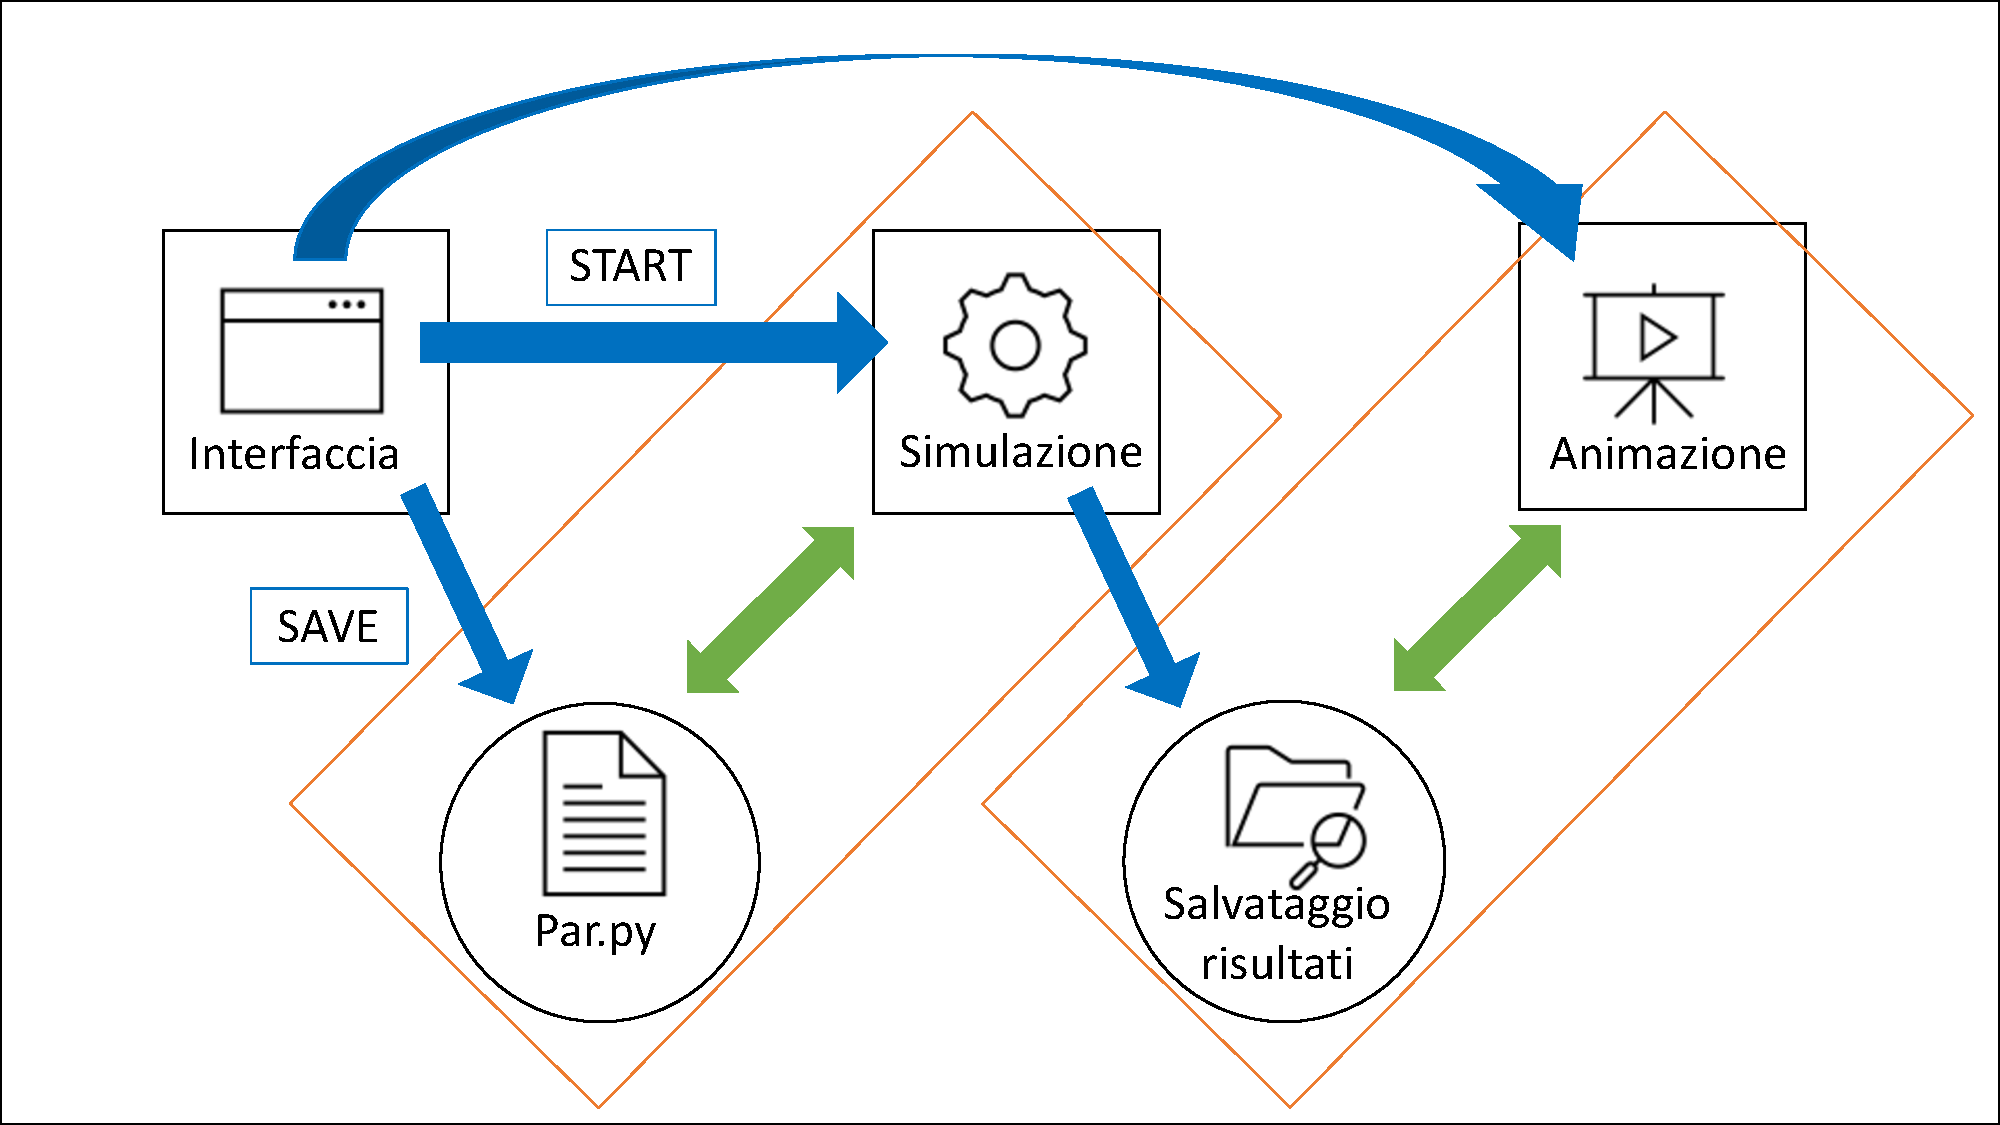
\includegraphics[width = 0.9\textwidth]{immagini/schema.pdf}
    \caption{ \textcolor{dark-gray}{Schema di funzionamento del software.}}
    \label{fig:schema}
\end{figure}

\section{Algoritmo di simulazione}
\label{sec:ev_code} 

Il cuore dell'algoritmo di simulazione è un ciclo che richiama, ad ogni iterazione, una funzione di evoluzione e salva i risultati nella cartella indicata dall'utente.
Sono state implementate tre diverse funzioni di evoluzione che differiscono per generalità e prestazioni. Inoltre l'utente può scegliere tra due tipologie di algoritmi di simulazione: con o senza anteprima, dove con anteprima si intende una visualizzazione in diretta dei risultati della simulazione. Questa scelta è dovuta alla diminuzione di velocità causata dalla creazione immediata dei grafici.
Di seguito si riporta il codice utilizzato per la più generica funzione di evoluzione, con la quale è possibile simulare un potenziale dipendente dal tempo e selezionare l'ordine a cui viene troncata l'espansione dell'eq.(\ref{eq:LT_expantion}). Per interpretare il codice si faccia riferimento al capitolo(\ref{ch:teoria}).
\newpage
\begin{lstlisting}[language = Python]
@jit                            # Comando al compilatore Numba

def evolution_t_dependent(  
                            y,      # Stato da evolvere
                            q,      # Vettore delle coordinate
                            k,      # Vettore dei momenti
                            dt,     # Grandezza del salto temporale
                            V,      # Vettore del potenziale
                            m,      # massa (parametro reale)
                            N,      # Numero di punti
                            L,      # Lunghezza dello spazio delle 
                                    #   coordinate
                            h,      # Valore di h tagliato
                            P_MAX,  # Valore massimo nello spazio 
                                    # dei momenti  
                            
                            coefficients, # Vettore dei coefficienti 
                                          #   dell'espansione
                            Level   # Ordine dell'espansione

                            mat_f,  #
                            mat_i,  # Matrici per il calcolo
                                    #    delle trasformate

                            f_zero, # Variabile di appoggio
                            ):         
    
    
    for i in range(Level):      # Questo ciclo rappresenta la
                                # produttoria nell'espansione
        
        if coefficients[i][0] != 0:     # Se c_i diverso da 0
                                        # applica il termine 
                                        # dipendente da V

            y = exp_V(y, V, dt, h, coefficients[i][0])
    
        if coefficients[i][1] != 0:     # Se d_i diverso da 0
                                        # applica il termine 
                                        # dipendente da T, ma 
                                        # nello spazio dei momenti
            
            # Applica la trasformata di Fourier
            f_y = DFT.Dft(y ,q, k, mat_f, N, L, h, f_zero)   

            # Trasla la soluzione per costruire la vera
            # rapprensetazione fisica nello spazio dei momenti
            f_y = DFT.shift(f_y, k, P_MAX)
            k = DFT.shift_p(k, P_MAX)

            # Applica il termine dipendente da T
            f_y = exp_T(f_y, k, m, dt, h, coefficients[i][1])
            
                                        # Riporta la funzione 
                                        # nello spazio delle 
                                        # coordinate

            # Trasla la funzione per poter utilizzare 
            # l'antitrasformta discreta
            f_y = DFT.back_shift(f_y, k)
            k = DFT.back_shift_p(k, P_MAX)

            # Applica l'antitrasformata di Fourier
            y= DFT.iDft(f_y, q, k, mat_i, L, h, f_zero)
            
            # Rincomincia il ciclo 

    return y

\end{lstlisting}
Il simbolo \textsl{@jit} è detto \textsl{decorator} e serve per compilare la funzione attraverso Numba. Tale processo rende il calcolo molto più rapido, ma per poter sfruttare al meglio le potenzialità di questo compilatore bisogna rinunciare ad alcune comodità tipiche dei linguaggi interpretati come Python. Numba richiede, infatti, che tutte le variabili utilizzate nella funzione siano passate come parametri e che le variabili siano di tipo statico. Per questo vengono inseriti tra i parametri alcuni termini che non hanno a che fare con l'evoluzione del sistema, ma che sono utilizzati come variabili di appoggio, come ad esempio \textsl{f\_zero}.
DFT è la libreria personale utilizzata per raggruppare i metodi che calcolano la trasformata di Fourier. Si ricorda che per poter applicare i termini a cui esponente compare $\hat{T}$ oltre che applicare la trasformata di Fourier è anche necessario traslare la soluzione. Questo viene fatto tramite i metodi \textsl{shift}, descritti nella sezione (\ref{sec:DFT}). Per rendere il codice più efficiente, le matrici, \textsl{mat\_f} e \textsl{mat\_i}, utilizzate per calcolare le trasformate, sono precalcolate e vengono passate alle funzioni come parametri.
Il parametro \textsl{coefficients} rappresenta un vettore di dimensioni $Level \times 2$ che raggruppa i coefficienti $c_j$ e $d_j$ dell'espansione nell'eq.(\ref{eq:LT_expantion}). 
Le funzioni \textsl{exp\_V} e \textsl{exp\_T} restituiscono i termini esponenziali che compaiono nell'espansione dell'eq.(\ref{eq:LT_expantion}). La funzione può essere resa più efficiente in quei casi in cui è possibile precalcolare alcuni termini. Per i potenziali non dipendenti dal tempo, infatti, i risultati restituiti dalle funzioni \textsl{exp\_V} e \textsl{exp\_T} sono sempre gli stessi. Quindi risulta più efficiente precalcolari e passarli come parametri, in modo da dover eseguire solo una moltiplicazione. Con questa modifica si ottiene la seconda versione della funzione di evoluzione.
Inoltre rinunciando alla scelta del livello di approssimazione si può migliorare ulterioremente l'efficienza della funzione rendendo più rapida la fase di compilazione. Nel codice è stato implementata una funzione di quest'ultimo tipo per il livello che corrisponde a troncare l'espansione a $\mathcal{O}(\delta t^{\, 3})$, cioè per l'espansione nell'eq.(\ref{eq:LT_2}). Si è scelto questo livello poiché è condierato, tra i tre proposti, il miglior compromesso tra precisione e costo computazionale. 

\begin{figure}
    \centering
    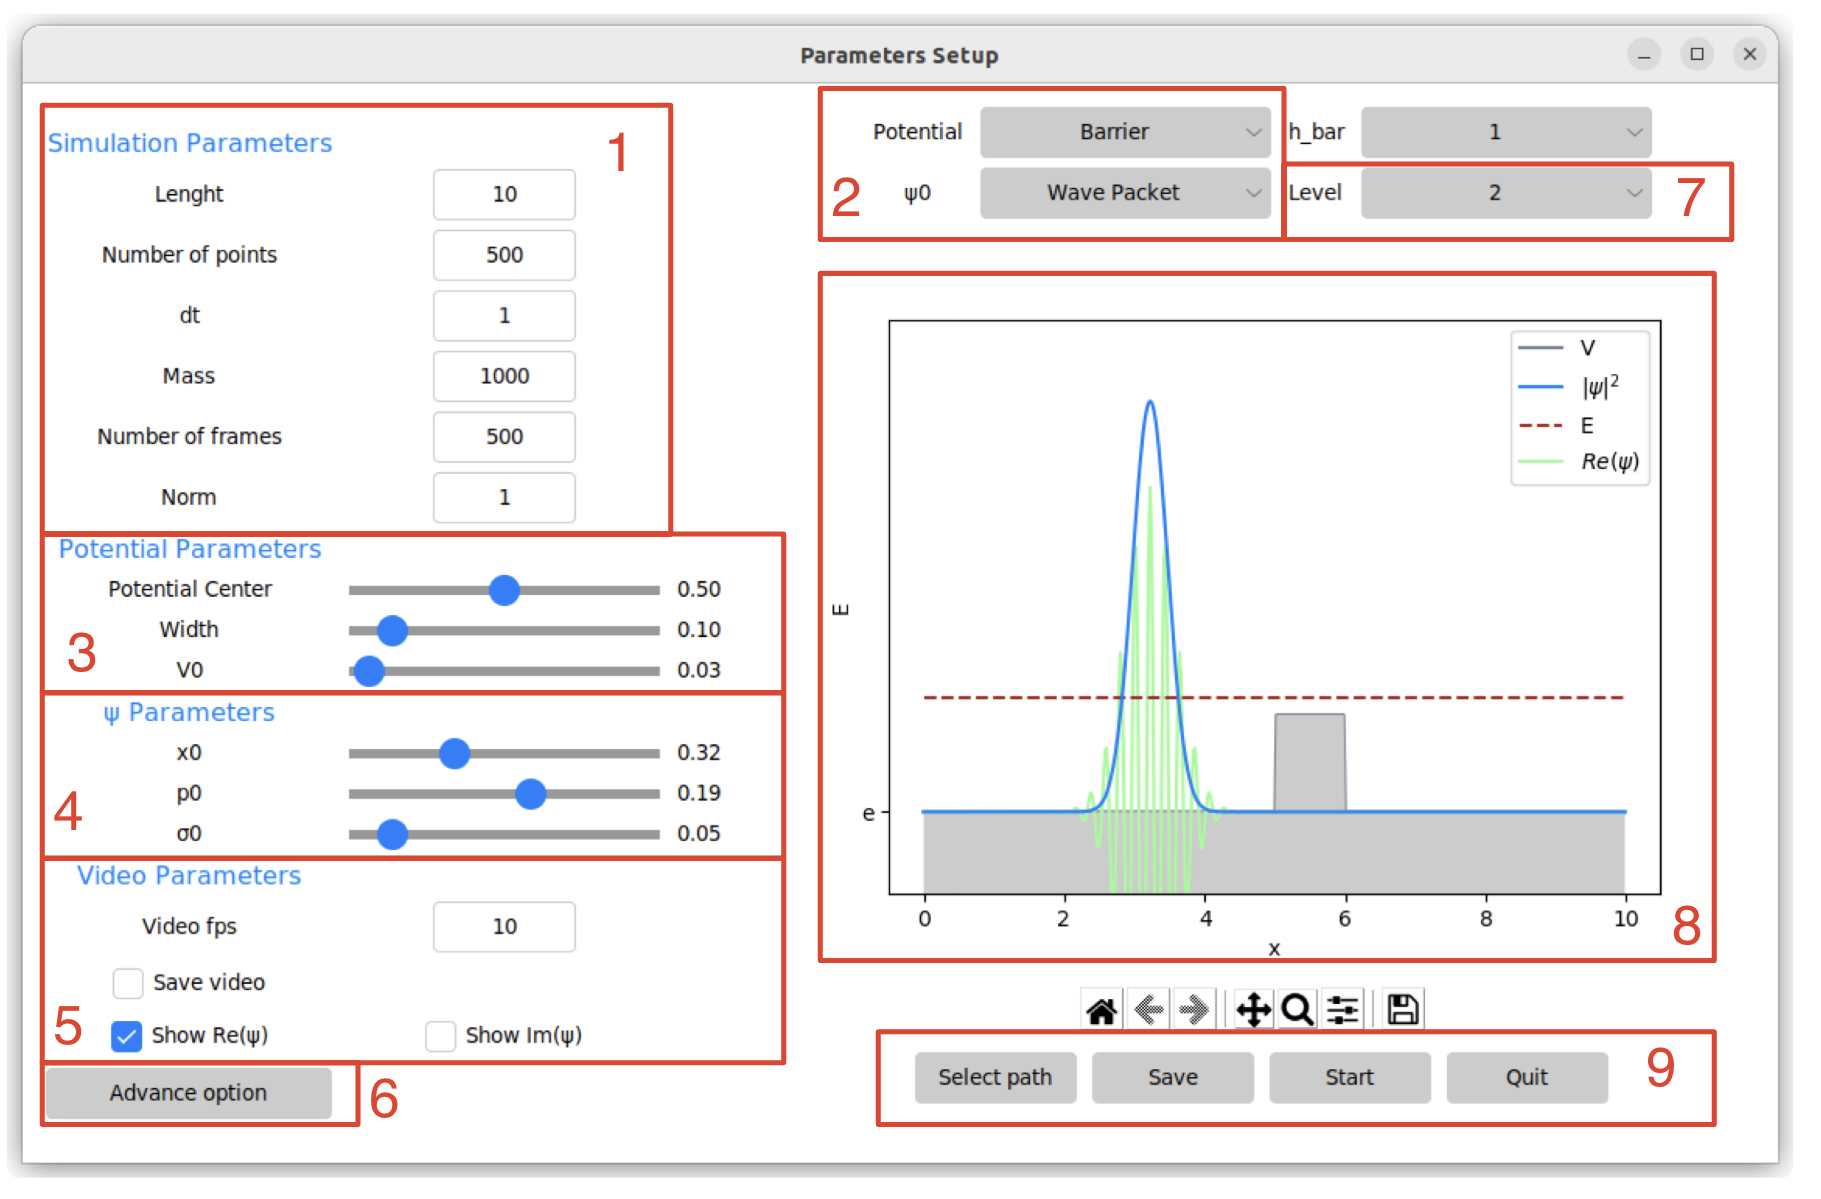
\includegraphics[width = \textwidth]{immagini/inter_num.jpg}
    \captionsetup{singlelinecheck=off}
    \caption[foo bar]{Illustrazione dell'interfaccia.

    \begin{enumerate}[nolistsep]
        \item Si possono modificare i parametri caratteristici dello spazio e della particella, nonché impostare il numero e la grandezza dei passi temporali da eseguire.
        \item Permette di scegliere tra gli stati e i potenziali riassunti nel capitolo(\ref{ch:applicazioni}).
        \item È possibile modificare i parametri caratteristici del potenziale selezionato.
        \item È possibile modificare i parametri caratteristici dello stato iniziale selezionato. Quando si modificano parametri che influenzano la funzione d'onda nello spazio dei momenti viene messa in mostra un'anteprima dello stato iniziale nello spazio dei momenti. 
        \item  Si possono modificare alcuni parametri per la creazione dell'animazione finale. Tra questi è possibile mostrare la parte reale e immaginaria della soluzione.
        \item Tra le opzioni avanzate si può selezionare l'algoritmo di simulazione, vedi sezione (\ref{sec:ev_code}), e inserire dei controlli per la conservazione della norma e dell'energia.
        \item Il parametro  \textsl{Level} indica l'ordine a cui viene troncata l'espansione nell'eq.(\ref{eq:LT_expantion}).
        \item Viene visualizzata in diretta un'anteprima dello stato iniziale.
        \item Cliccando su questi tasti si controllano le funzioni dell'interfaccia. Per eseguire in maniera corretta la simulazione la procedura prevista è: selezionare il percorso di salvataggio, salvare i risultati, far partire la simulazione e attendere l'animazione, uscire.    
    \end{enumerate}
    }
    \label{fig:interface}
\end{figure}

\clearpage

\addcontentsline{toc}{chapter}{Conclusioni} % Capitolo non numerato

\chapter*{Conclusioni}
\label{ch:conclusioni}

Grazie al lavoro esposto nella sezione (\ref{ch:Validazione}) è possibile affermare che la soluzione numerica
%cambia
generata tramite la simulazione è  del tutto compatibile con la soluzione esatta. 
È quindi possibile utilizzare questo strumento per risolvere un qualsiasi problema monodimensionale e ottenere risultati concreti, come nella sezione (\ref{ch:applicazioni}). 

%amplia
Il formalismo esposto nella sezione (\ref{ch:teoria}) è dunque verificato e applicato. Tale formalismo è generalizzabile per qualsiasi operatore $\hat{H}$, che sia somma di due operatori non commutanti, in un numero arbitario di dimensioni. I problemi che si possono riscontrare nella generalizzazione riguardano soprattutto il costo computazionale e le strategie di visualizzazione dei risultati. Ogni volta che si aumentano le dimensioni o i gradi di libertà del sistema (ad esempio considerando lo spin), è necessario ampliare la grandezza dei vettori che contengono la funzione d'onda. Nello spazio delle coordinate l'aumento di punti da considerare scala con $N^d$, dove $d$ rappresenta il numero di dimensioni. Inoltre per rappresentare funzioni d'onda multidimensionali è necessario animare uno spazio tridimensionale o quadridimensionale, il che, anche se possibile, rende i risultati più difficili da visualizzare. 

\chapter*{Ringraziamenti}
Vorrei dedicare qualche riga a coloro che mi hanno accompagnato in questo percorso.

Vorrei innanzitutto ringraziare il mio relatore Carlo Oleari, per la disponibilità e precisione dimostratemi durante tutto il periodo di stesura del lavoro di tesi. Grazie per avermi spinto con il suo esempio ad essere uno studente migliore, più curioso e più diligente. 

Ringrazio infinitamente i miei genitori che mi hanno sempre sostenuto, appoggiando ogni mia decisione, fin dalla scelta del mio percorso di studi e senza i quali non sarei qui oggi.

Ringrazio la mia fidanzata Lucia per avermi dato la forza e il coraggio per affrontare tutto questo. Grazie per tutto il tempo che mi hai dedicato. Grazie perché ci sei sempre stata. 

Grazie a tutti i colleghi ed amici che ho conosciuto in questi anni e con cui ho condiviso alcuni dei momenti più importanti della mia vita. Grazie per avermi accolto nel vostro gruppo e aiutato anche nei periodi più difficili. 

\printbibliography
\nocite{*}

\end{document}
